% !Mode:: "TeX:UTF-8"
%%%%%%%%%%%%%%%%%%%%%%%%%%%%%%%%%%%%%%%%%%%%%%%%%%%%%%%%%%%%%%%%%%%%%%%%%%%%%%%%
%          ,
%      /\^/`\
%     | \/   |                CONGRATULATIONS!
%     | |    |             SPRING IS IN THE AIR!
%     \ \    /                                                _ _
%      '\\//'                                               _{ ' }_
%        ||                     hithesis v3                { `.!.` }
%        ||                                                ',_/Y\_,'
%        ||  ,                   dustincys                   {_,_}
%    |\  ||  |\          Email: yanshuoc@gmail.com             |
%    | | ||  | |            https://yanshuo.site             (\|  /)
%    | | || / /                                               \| //
%    \ \||/ /       https://github.com/dustincys/hithesis      |//
%      `\\//`   \\   \./    \\ /     //    \\./   \\   //   \\ |/ /
%     ^^^^^^^^^^^^^^^^^^^^^^^^^^^^^^^^^^^^^^^^^^^^^^^^^^^^^^^^^^^^^^
%%%%%%%%%%%%%%%%%%%%%%%%%%%%%%%%%%%%%%%%%%%%%%%%%%%%%%%%%%%%%%%%%%%%%%%%%%%%%%%%
\documentclass[type=bachelor,campus=harbin]{hithesisbook}
% 此处选项中不要有空格
%%%%%%%%%%%%%%%%%%%%%%%%%%%%%%%%%%%%%%%%%%%%%%%%%%%%%%%%%%%%%%%%%%%%%%%%%%%%%%%%
% 必填选项
% type=doctor|master|bachelor|postdoc
%%%%%%%%%%%%%%%%%%%%%%%%%%%%%%%%%%%%%%%%%%%%%%%%%%%%%%%%%%%%%%%%%%%%%%%%%%%%%%%%
% 选填选项(选填选项的缺省值已经尽可能满足了大多数需求,除非明确知道自己有什么
% 需求)
% campus=shenzhen|weihai|harbin
%   含义:校区选项,默认harbin
% glue=true|false
%   含义:由于我工规范中要求字体行距在一个闭区间内,这个选项为true表示tex自
%   动选择,为false表示区间内一个最接近版心要求行数的要求的默认值,缺省值为
%   false。
% tocfour=true|false
%   含义:是否添加第四级目录,只对本科文科个别要求四级目录有效,缺省值为
%   false
% fontset=windows|mac|ubuntu|fandol|adobe
%   含义:设置字体,若不指定会自动识别系统,然后设置字体。fandol是开源字体,自行
%   下载安装后设置使用。windows是中易字库,窝工默认常用字体,绝对没毛病。mac和
%   ubuntu 默认分别是华文和思源字库,理论上用什么字库都行。后两种字库的安装方法
%   到谷歌上百度一下什么都有了。Linux非ubuntu发行版、非x86架构机器等如何运行可到
%   github issue上讨论。
% tocblank=true|false
%   含义:目录中第一章之前,是否加一行空白。缺省值为true。
% chapterhang=true|false
%   含义:目录的章标题是否悬挂居中,规范中要求章标题少于15字,所以这个选项
%   有无没什么用,除了特殊需求。缺省值为true。
% fulltime=true|false
%   含义:是否全日制,缺省值为true。非全日制如同等学力等,要在cover中设置类
%   型,封面中不同格式
% subtitle=true|false
%   含义:论文题目是否含有副标题,缺省值为false,如果有要在cover中设置副标
%   题内容,封面中显示。
% newgeometry=one|two|no
%   含义:规范中的自相矛盾之处,版芯是否包含页眉页脚,旧方法是按照包含页眉
%   页脚来设置。该选项是多选选项,如果设置为no,则版新为旧模板的版芯设置方法,
%   如果设置该选项one或two,分别对应两种页眉页码对应版芯线的相对位置。第一种
%   是严格按照规范要求,难看。第二种微调了页眉页码位置,好一点。默认two。
% debug=true|false
%   含义:是否显示版芯框和行号,用来调试。默认否。
% openright=true|false
%   含义:博士论文是否要求章节首页必须在奇数页,此选项不在规范要求中,按个
%   人喜好自行决定。 默认否。注意,窝工的默认情况是打印版博士论文要求右翻页
%   ,电子版要求非右翻页且无空白页。如果想DIY(或身不由己DIY)在什么地方右
%   翻页,将这个选项设置为false,然后在目标位置添加`\cleardoublepage`命令即
%   可。
% library=true|false
%   含义:是否为提交到图书馆的电子版。默认否。注意:如果设置成true,那么
%   openright选项将被强制转换为false。
% capcenterlast=true|false
%   含义:图题、表题最后一行是否居中对齐(我工规范要求居中,但不要求居中对
%   齐),此选项不在规范要求中,按个人喜好自行决定。默认否。
% subcapcenterlast=true|false
%   含义:子图图题最后一行是否居中对齐(我工规范要求居中,但不要求居中对齐
%   ),此选项不在规范要求中,按个人喜好自行决定。默认否。
% absupper=true|false
%   含义:中文目录中的英文摘要在中文目录中的大小写样式歧义,在规范中要求首
%   字母大写,在work样例中是全大写。该选项控制是否全大写。默认否。
% bsmainpagenumberline=true|false
%   含义:由于本科生论文官方模板的页码和页眉格式混乱,提供这个选项自定义设
%   置是否在正文中显示页码横线,默认显示。
% bsfrontpagenumberline=true|false
%   含义:由于本科生论文官方模板的页码和页眉格式混乱,提供这个选项自定义设
%   置是否在前文中显示页码横线,默认显示。
% bsheadrule=true|false
%   含义:由于本科生论文官方模板的页码和页眉格式混乱,提供这个选项自定义设
%   置是否显示页眉横线,默认显示。
% splitbibitem=true|false
%   含义:参考文献每一个条目内能不能断页,应广大刀客要求添加。默认否。
% newtxmath=true|false
%   含义:数学字体是否使用新罗马。默认是。
% chapterbold=true|false
%   含义:本科生章标题在目录和正文中是否加粗
% engtoc=true|false
%   含义:非博士生需要添加英文目录的,手动添加,如果是博士,此开关无效
% zijv=word|regu
%   含义:字距设置为规范规定33个字还是word中34个字。默认regu。
% citetwo=comma|endash
%   含义:相邻两个参考文献中的连接符是由逗号:[1,2]还是短线[1-2]。默认endash
%%%%%%%%%%%%%%%%%%%%%%%%%%%%%%%%%%%%%%%%%%%%%%%%%%%%%%%%%%%%%%%%%%%%%%%%%%%%%%%%
\usepackage{hithesis}

\graphicspath{{figures/}}

\begin{document}
\frontmatter
% !Mode:: "TeX:UTF-8"

\hitsetup{
  %******************************
  % 注意:
  %   1. 配置里面不要出现空行
  %   2. 不需要的配置信息可以删除
  %******************************
  %
  %=====
  % 秘级
  %=====
  statesecrets={公开},
  natclassifiedindex={TM301.2},
  intclassifiedindex={62-5},
  %
  %=========
  % 中文信息
  %=========
ctitleone={高性能RISC-V开源处理},%本科生封面使用
ctitletwo={器虚拟化扩展与系统评测},%本科生封面使用
  ctitlecover={高性能RISC-V开源处理器\\虚拟化扩展与系统评测},%放在封面中使用,自由断行
  ctitle={高性能RISC-V开源处理器虚拟化扩展与系统评测},%放在原创性声明中使用
  % csubtitle={一条副标题}, %一般情况没有,可以注释掉
  cxueke={工学},
  csubject={计算机科学与技术},
  caffil={计算学部},
  cauthor={胡光辉},
  csupervisor={黄庆成副教授},
  cassosupervisor={某某某教授}, % 副指导老师
  ccosupervisor={某某某教授}, % 联合指导老师
  % 如果是深圳本科毕业论文,需要取消注释下一行,并将内容改为“规范”中要求的封面第一页最下方的日期
% szshortcdate={2024年6月},
  % 日期自动使用当前时间,若需指定按如下方式修改:
  %cdate={超新星纪元},
  cstudentid={120L052208},
  % cstudenttype={学术学位论文}, %非全日制教育申请学位者
  % cnumber={no9527}, %编号
  % cpositionname={哈铁西站}, %博士后站名称
  % cfinishdate={20XX年X月---20XX年X月}, %到站日期
  % csubmitdate={20XX年X月}, %出站日期
  % cstartdate={3050年9月10日}, %到站日期
  % cenddate={3090年10月10日}, %出站日期
  %(同等学力人员)、(工程硕士)、(工商管理硕士)、
  %(高级管理人员工商管理硕士)、(公共管理硕士)、(中职教师)、(高校教师)等
  %
  %
  %=========
  % 英文信息
  %=========
  etitle={Research on key technologies of partial porous externally pressurized gas bearing},
  esubtitle={This is the sub title},
  exueke={Engineering},
  esubject={Computer Science and Technology},
  eaffil={\emultiline[t]{School of Mechatronics Engineering \\ Mechatronics Engineering}},
  eauthor={Yu Dongmei},
  esupervisor={Professor XXX},
  eassosupervisor={XXX},
  % 日期自动生成,若需指定按如下方式修改:
  edate={December, 2017},
  estudenttype={Master of Art},
  %
  % 关键词用“英文逗号”分割
  ckeywords={\TeX, \LaTeX, CJK, 嗨!, thesis},
  ekeywords={\TeX, \LaTeX, CJK, template, thesis},
}

\begin{cabstract}

  摘要的字数(以汉字计),硕士学位论文一般为500 $\sim$ 1000字,博士学位论文为1000 $\sim$ 2000字,
  均以能将规定内容阐述清楚为原则,文字要精练,段落衔接要流畅。摘要页不需写出论文题目。
  英文摘要与中文摘要的内容应完全一致,在语法、用词上应准确无误,语言简练通顺。
  留学生的英文版博士学位论文中应有不少于3000字的“详细中文摘要”。
  
  关键词是为了文献标引工作、用以表示全文主要内容信息的单词或术语。关键词不超过 5
  个,每个关键词中间用分号分隔。(模板作者注:关键词分隔符不用考虑,模板会自动处
  理。英文关键词同理。)
\end{cabstract}

\begin{eabstract}
  An abstract of a dissertation is a summary and extraction of research work
  and contributions. Included in an abstract should be description of research
  topic and research objective, brief introduction to methodology and research
  process, and summarization of conclusion and contributions of the
  research. An abstract should be characterized by independence and clarity and
  carry identical information with the dissertation. It should be such that the
  general idea and major contributions of the dissertation are conveyed without
  reading the dissertation.
  
  An abstract should be concise and to the point. It is a misunderstanding to
  make an abstract an outline of the dissertation and words ``the first
  chapter'', ``the second chapter'' and the like should be avoided in the
  abstract.
  
  Key words are terms used in a dissertation for indexing, reflecting core
  information of the dissertation. An abstract may contain a maximum of 5 key
  words, with semi-colons used in between to separate one another.
\end{eabstract}
 % 封面
\makecover
% % !TEX root = ../main.tex

% 物理量符号表,如果采用标准符号则不需要此表
\begin{denotation}
  % 此处最好是h
  \begin{table}[h]
  \caption{国际单位制中具有专门名称的导出单位}
  \vspace{0.5em}\centering\wuhao
  \begin{tabular}{ccccc}
    \toprule[1.5pt]
    量的名称&单位名称&单位符号&其它表示实例\\
    \midrule[1pt]
    频率&赫[兹]&Hz&s-1\\
    \bottomrule[1.5pt]
    \end{tabular}
  \end{table}
\end{denotation}
%物理量名称表,符合规范为主,有要求添加
\tableofcontents %目录
\mainmatter
% !TEX root = ../main.tex
\chapter{绪论}[Introduction]
虚拟化技术,作为计算机科学领域的一项关键技术,为云数据中心提供的各类服务构建了核心的技术框架。
随着近年来云数据中心及云服务提供商的快速发展,从初期的虚拟机与容器技术,
到新兴的函数即服务(Function as a Service, FaaS)与无服务器计算(serverless computing)模式,
均展现出了强烈的市场需求和广阔的发展潜力。
这一趋势不断促进虚拟化技术的进步与创新,尤其是在处理器虚拟化领域。
处理器虚拟化技术,作为实现硬件兼容性的重要手段之一,使得虚拟机能够在与底层物理硬件架构完全不同的环境下运行不同操作系统,从而在云计算服务中扮演着至关重要的角色。

经过多年的深入研究,尤其是在需求驱动的影响下,
关于虚拟化技术及其评估方法的探讨,特别是在x86和ARM体系架构上,已经达到了高度成熟的阶段。
然而,当我们转向RISC-V,这个新兴的开源精简指令集,我们发现其处理器虚拟化技术的研究仍处于起步阶段,研究潜力巨大。RISC-V凭借其简洁、高效以及模块化的特性,在计算机体系架构领域受到了学术界和工业界的广泛瞩目。
为了实现处理器的虚拟化,RISC-V推出了一种新的指令集扩展——虚拟化扩展(Hypervisor Extension)。
该扩展明确规定了实现处理器虚拟化所必需的硬件功能,其中包括特权指令和页表翻译等关键技术。

关于RISC-V虚拟化扩展的研究,加州大学的伯克利分校迈出了第一步。
他们研发了Rocket Chip,一个开源的RISC-V顺序流水线处理器,
并在其上实现了完整的虚拟化扩展,进行了一系列虚拟化相关的评测。
但是在真实应用场景下,硬件情况会更为复杂,
多核乱序的处理器核心才是虚拟化服务器的主流。
关于这方面的研究尚未完全展开,亟待进行。
\chapter{技术背景及研究动机}

本章首先介绍RISC-V虚拟化扩展,特别是虚拟内存部分提出的第二阶段地址翻译。
第二,介绍“香山”处理器的内存管理单元的原始架构。
在第三章会直接介绍虚拟化扩展下的内存管理单元,此处对原始架构的说明能够帮助理解。
第三,介绍本项目所使用的所有调试工具和评测平台,能够帮助后文实验部分的理解。
最后,会结合虚拟化扩展硬件实现的相关研究,介绍本项目的研究动机。

\section{RISC-V虚拟化扩展}
RISC-V的虚拟化扩展需要添加的硬件功能大致可分为特权控制和虚拟内存两大部分。
在特权控制方面,主要新增了3种特权模式、12条特权指令、23个控制状态寄存器以及虚拟化相关的4种中断和6种异常。
在虚拟内存方面,首先定义了第二阶段地址翻译的概念,
同时添加了上述部分的控制状态寄存器、虚拟内存管理指令和异常,为程序员提供了管理第二阶段地址翻译的手段。

\paragraph{特权控制}
特权等级在未支持虚拟化扩展时只有机器模式(M-mode)、监管模式(S-mode)和用户模式(U-mode)。
分别对应标准体系结构中运行引导程序,操作系统和用户程序的机器状态。
虚拟化扩展下的特权等级变化如图\ref*{fig:priv-mode},原本的监管模式被改成虚拟机管理模式(HS-mode),对应于虚拟机管理程序的层级。
还新增了虚拟监管模式(VS-mode)和虚拟用户模式(VU-mode),对应于虚拟机和虚拟机下的用户态程序。
此外还保留了原始的用户模式,对应于Type2虚拟机监管系统下的宿主操作系统的用户程序。
例如在Linux KVM中,需要先启动宿主Linux操作系统,此时处理器运行在虚拟机管理模式下。
在宿主操作系统除了具有启动虚拟机的功能,还具有一般Linux操作系统的所有能力。
在未启动虚拟机时运行的用户态程序时,处理器就在用户模式下,而不是虚拟用户模式。

\begin{figure}[htbp]
    \centering
    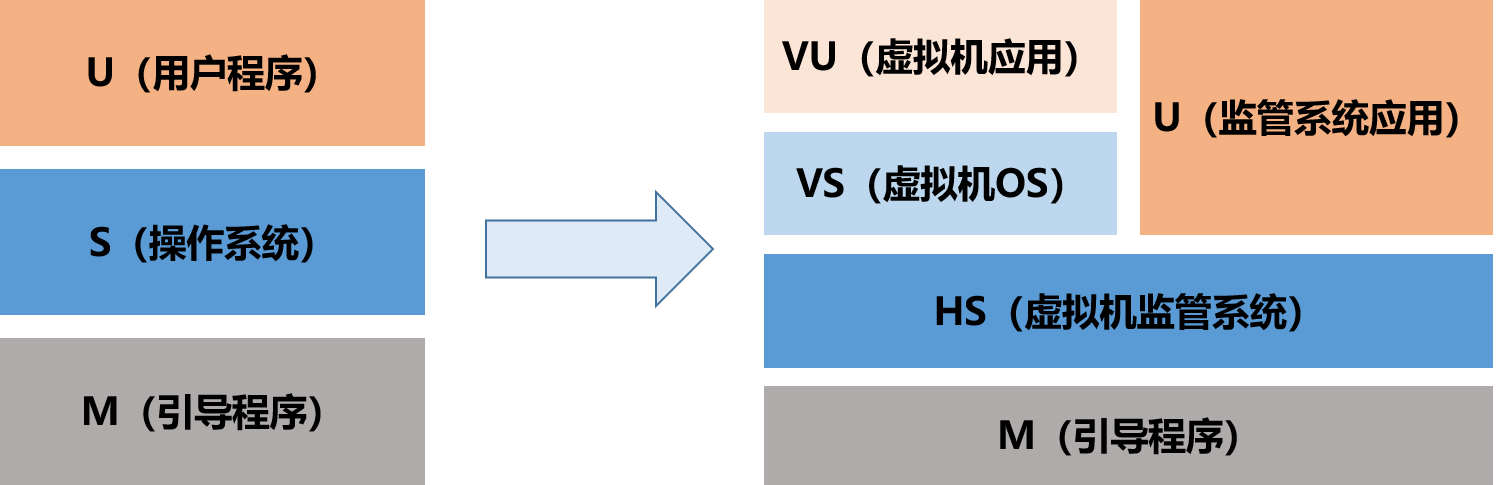
\includegraphics{priv-mode.png}
    \caption{RISC-V虚拟化扩展特权等级变化}
    \label{fig:priv-mode}
\end{figure}

控制管理寄存器(Control Status Register,CSR)是RISC-V处理器中的一组特殊寄存器,
用于控制处理器的行为和存储处理器的状态信息。
这些寄存器包含了处理器的核心控制逻辑和状态信息,可以被软件访问和操作。
虚拟化扩展下,控制管理寄存器的一个最主要的变化是添加了一套在虚拟监管模式下使用的,
用于处理虚拟机中的异常自陷的流程的寄存器,例如配置自陷地址的vstvec、保存异常指令地址的vsepc。
分离管理系统和虚拟机中使用的配置寄存器,能够使得虚拟机中出现异常时可以自己处理,不必自陷到虚拟机管理系统中。
另一个变化是添加了一些虚拟机管理系统使用寄存器,用于配置管理系统可以捕获的虚拟机内执行的特殊指令(hstatus),
虚拟机的中断注入和委托(hedeleg、hideleg、hgeip、hgeie)等。
因此,在中断异常的种类方面,原始的监管模式下所有的中断被虚拟机管理模式和虚拟监管模式各复制一份,
虚拟机管理模式还需要添加一个虚拟机外部中断,用于实现虚拟机直通中断。

最后一部分是虚拟机管理模式下的特权指令和新增的页错误异常,为程序员提供管理虚拟地址翻译的方法。
在未实现虚拟化扩展下的SFENCE.VMA指令用于同步页表数据结构,相对的,虚拟化扩展下新增了HFENCE.VVMA和HFENCE.GVMA,
用于第二阶段地址翻译的页表数据结构的同步。
同时新增了HLV.width, HLVX.HU/WU, HSV.width指令,为虚拟机管理系统提供了读取虚拟机内存的方法。

\paragraph{虚拟内存}
第二阶段地址翻译是虚拟化扩展提出的重要概念,是指在虚拟化环境中进行的地址转换过程的第二个阶段。
在传统的虚拟地址翻译机制中,虚拟地址(Virtual Address)只需要经过一次多级页表翻译
即可成为物理地址(Physical Address)访问实际的内存。
在第二段地址翻译开启时,虚拟机操作系统会对内部的虚拟地址进行一次页表翻译,
即将虚拟机虚拟地址(Guest Virtual Address,GVA)翻译成虚拟机物理地址(Guest Physical Address,GPA)。
此时处理器还需要再进行一次多级地址翻译
将虚拟机物理地址翻译成主机物理地址(Host Physical Address,HPA)才能够访问内存。
图\ref*{fig:Sv39x4}以经典的三级页表——Sv39为例,展示了两者的关系。
未开启第二阶段翻译时,例如虚拟机管理程序运行时,
最多需要访问内存三次,获取三个页表项(Page Table Entry)即可完成地址翻译。
但在开启第二阶段地址翻译后,例如在虚拟监管模式下运行虚拟机,
每次访存获取下一级页表之前,都需要再经过三级页表翻译。
换言之,为了获得虚拟机的虚地址所对应的物理地址,最多需要12次的内存访问。

\begin{figure}[htbp]
    \centering
    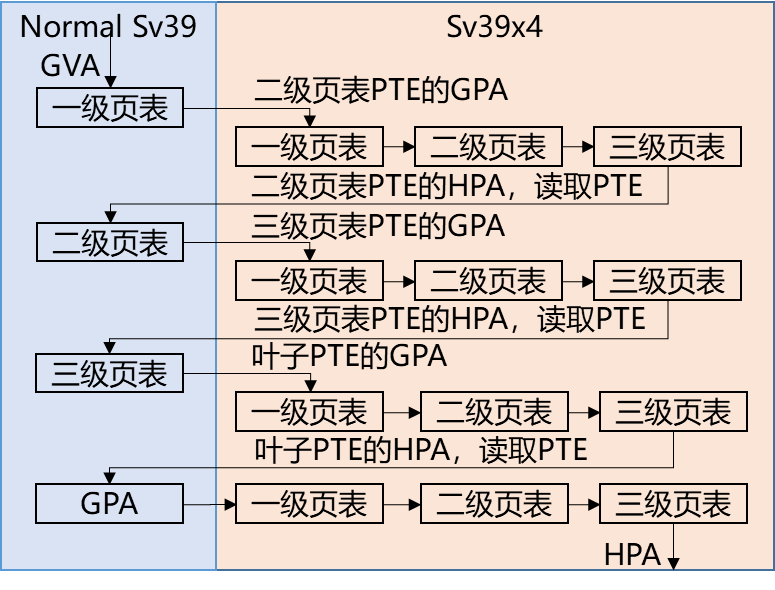
\includegraphics[scale=0.8]{Sv39x4.png}
    \caption{RISC-V虚拟化扩展的两阶段地址翻译}
    \label{fig:Sv39x4}
\end{figure}

为了管理第二阶段的地址翻译的相关信息,处理器需要提供相应的指令和控制状态寄存器用于配置。
关于控制状态寄存器,首先是第二阶段地址翻译的叶目录的根地址,保存在hgapt的寄存器中,对应于保存第一阶段地址翻译相关信息的sapt寄存器。
其次,在地址翻译的过程中不免要进行访存和权限检查,如果失败会导致处理器产生一个页错误的异常,用于操作系统进行替换或者进一步的诊断。
因此,虚拟化扩展新增了虚拟机物理页错误的异常,对应于第二阶段地址翻译时的权限检查失败或者访存错误。
自然的,虚拟机物理页错误异常的处理程序需要触发异常的虚拟机物理地址进行诊断,htval和mtval2寄存器被新增用于在异常触发时保存虚拟机物理地址。
可以预见,处理器的流水线内部同样需要空间保存错误地址。
特别对于取指时触发的虚拟机页错误异常,需要该指令携带地址直至退休,这对流水线中的存储部件来说是一种较大的面积开销。
对于虚拟内存管理指令,在上文也有提及。用于同步第二阶段页表翻译单元数据结构的HFENCE.VVMA和HFENCE.GVMA指令。
一个简单的实现可以是无效处理器内有关第二阶段地址翻译的所有缓存。
关于HLV.width, HLVX.HU/WU, HSV.width指令,实质是在虚拟机管理模式下开启第二阶段地址翻译进行访存。

\section{“香山”处理器的内存管理单元}
未实现虚拟化扩展的“香山”处理器的内存管理单元的整体结构如图\ref{fig:origin-mmu}所示,可分为如下两部分:
分布式的一级页表缓存(Level 1 Translation Lookaside Buffer,L1 TLB)和
集中式的地址映射引擎(Address Mapping Enging, AME),主要包括页表翻译单元(Page Table Walker)和
二级页表缓存(Level 2 Translation Lookaside Buffer,L2 TLB)。

\begin{figure}[htbp]
    \centering
    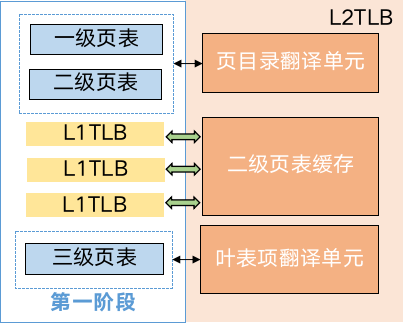
\includegraphics[scale=0.6]{origin-mmu.png}
    \caption{“香山”处理器原始内存管理单元架构}
    \label{fig:origin-mmu}
\end{figure}

\paragraph{一级页表缓存} 一级页表缓存分布在处理器各个需要地址翻译的流水线中,例如前端的指令缓存、指令预取,后端的访存流水线。
一级页表缓存的缓存条目记录虚地址对应的多级页表翻译后的最终物理地址,因此可以实现地址翻译请求的快速的回应。
缓存条目的组织方式是全相连映射,同时每个缓存条目由使用直接映射的组织方式,存储了多个翻译结果。

\paragraph{地址映射引擎} 当一级页表缓存不命中时,会发送翻译请求到地址映射引擎。
地址映射引擎包括一个大型的二级页表缓存、页表翻译单元、以及各种权限检查模块,例如PMP和PMA。
二级页表缓存的每个条目记录了虚地址对应的各级页表,可支持各级的地址翻译请求,
具体而言,包括4KB、2MB、1GB三种大小的页表。
当翻译请求无法在页表缓存中找到,翻译请求会发送至页表翻译单元,包括页目录翻译单元和叶表项翻译单元。
页目录翻译单元负责第一级页表和第二级页表的查询,是一个朴素的阻塞自动机实现。
叶表项翻译单元负责第三级页表的查询,使用猝发访存使用高并发。
二级页表缓存会根据请求的命中级数,将对应的翻译请求转发给对应的模块,尽可能减少实际的内存访问。
简而言之,二级页表缓存作为地址映射引擎的中心,负责一级页表缓存不命中时的三级页表翻译,
当二级页表缓存不命中时,会将请求转发给翻译单元,翻译单元通过访问内存,将翻译结果回填至二级页表缓存。

\section{处理器设计的调试及评测平台}
在传统的处理器设计流程中,常用的平台包括硬件描述语言(Hardware Description Language,HDL)建模、
逻辑分析仪(Logic Analyzer)、软件仿真工具(Simulation Tools)
和现场可编程逻辑门阵列(Field-Programmable Gate Array,FPGA)。
然而,这些方法存在一些局限性,导致开发效率较低。

在调试方面,逻辑分析仪的软件仿真可以帮助观测硬件设计在外界激励下的行为。
通过数学模型和计算机算法模拟硬件设计,获取设计中各个信号值随时间的变化曲线,即波形图。
尽管波形图和仿真软件可以帮助工程师了解电路内部的所有状态,是错误调试的基础,
但是当需要在各种复杂场景下进行调试时,仍旧存在许多缺陷。
首先,波形重放在发现错误信号的能力有限。
单一信号的微小错误会被淹没在巨大的细节中,很可能数千万个周期后的才会暴露。
因此,学术界近年来提出了使用架构模拟器和差分测试的方法\cite{micro2022xiangshan}。
通过比对正确的体系结构信息,精确定位出错现场。
其次,仿真工具由于其可并行性低、同步要求高等自身特性,必然导致了执行速度原低于FPGA。
尽管在开源社区和学术界存在许多高效的解决方案,
例如iverilog\cite{github:iverilog}、
verilator\cite{github:verilator}和manticore\cite{asplso23manticore}。
但在运行大型基准测试和系统软件时,花费的时间仍然不可接受。

在评测方面,FPGA被广泛运用于原型验证。
通过将处理器设计部署在物理的逻辑门和寄存器中,
FPGA能够提供更真实的测试环境和远快于软件仿真的运行速度。
同时,在FPGA中实现特定硬件的时间成本开销远小于通过流片方式生产的开销。
但是,FPGA由于其硬件特性,能够获取的波形信号和时间范围十分受限。
只能通过对外部设备的输出,判断硬件设计是否存在错误,无法提供调试所需的电路内部信息。
基于上述缺陷,学术界提出了一种通过FPGA加速软件仿真的方案——REMU\cite{iccd2023remu},
通过将FPGA某一运行时刻的所有寄存器和存储器信息,精确重放到仿真软件中。
利用仿真软件生成波形的能力来帮助调试。
本项目中也使用了该方法发现硬件设计的错误,提高了开发效率。

\section{虚拟化扩展的软硬件支持}
在RISC-V虚拟化拓展规范的仍处于草案阶段时,
一些主流虚拟机管理程序和模拟器就已经随着拓展的技术规范的更新进行适配,
例如Xvisor\cite{micro2022xiangshan}、KVM\cite{kvm:H-ext}
QEMU\cite{qemu-riscv:H-ext},Spike\cite{github:spike}等。
然而,关于虚拟化扩展的硬件实现,仅从拓展的0.6.1版本发布后才陆续出现。

虚拟化扩展的硬件实现工作最早开展在Rocket Chip\cite{itco2022rocket}中,这是加州大学伯克利分校开发的顺序单发射流水线处理器。
此外,该工作还在处理器中移植了Bao,一种轻量级的虚拟机管理系统\cite{ng-res2020bao},并且进行了一些简易的虚拟化性能评测。
2023年,一个六级流水的乱序单发射开源处理器核心CVA6\cite{tvlsi2023cva6}也实现了虚拟化扩展。
该工作不仅进行了关于两阶段地址转化技术的微架构探索,还对性能、功耗、面积等物理设计进行了一系列优化。

在商业界,StarFive发布了Dubhe系列,这是首款支持虚拟化的商业级RISC-V处理器IP核。
此外,SiFive的P600系列处理器也支持虚拟化扩展。
其他支持虚拟化扩展的处理器包括InCore Semiconductors的Chromite处理器和IIT Madras发布的Shakti处理器。
这些处理器提供了硬件级别的支持,使得虚拟化技术在RISC-V体系结构中得到了广泛应用。

\section{研究动机}

今天,云数据中心服务提供商在迅速地发展,市场中可见的各种云服务,其根本的底层技术都是处理器虚拟化。
在市场需求的刺激下,处理器芯片的主流架构,例如Intel和ARM都提供了虚拟化的硬件支持。
近年来,RISC-V作为一个新兴的开放指令集,也开始着手云数据中心的需求。
然而,如上文虚拟化扩展的软硬件支持所述,关于RISC-V处理器的虚拟化技术的研究还十分有限,
特别是高性能处理器在虚拟化扩展方面的相关研究。
尽管Rocket Chip和CVA6实现了虚拟化扩展,但他们都是单发射处理器。
因此,高性能RISC-V处理器的虚拟化扩展相关的研究亟待进行。
本项目尝试填补这一空缺,研究内容包括处理器硬件扩展到虚拟化软件,以及全系统的虚拟化性能评估。

硬件方面,本项目着手“香山”项目——目前国际上性能最高的RISC-V处理器核。
尝试在“香山”中实现虚拟化扩展,主要包括特级管理单元、内存管理单元的扩展。
特别是内存管理单元,本项目尝试了各种能够加快速度、提高吞吐量的微架构。
相比Rocket Chip的最朴素的实现,“香山”实现了支持VMID和ASID的虚拟内存屏障指令,
这能够减少屏障指令执行时无效化的缓存条目,加快地址翻译的速度。
CVA6实现了第二阶段专用的页表缓存,被称为GTLB,并表明该微架构能够加速第二阶段页表翻译单元的速度。
“香山”的微架构设计与其和而不同,通过在二级页表缓存存放两阶段的页表,
同时在进行第二阶段页表翻译前查询二级页表缓存。
该方案实现了类似的第二阶段专用是页表缓存的效果,而且最小化对原有设计的修改,没有额外的缓存面积开销。
尽管CVA6和Rocket Chip均实现了二级页表缓存,但“香山”是首个将二级页表缓存用于第二阶段页表的开源RISC-V处理器。
除此之外,“香山”在一级页表缓存以及页表翻译单元均有其他能够提高吞吐、加快速度的微架构设计。
这些设计对虚拟化性能能够产生何种效果,同样具有巨大的研究价值,能够为后来者提供了设计思路和经验。

虚拟化软件方面,本项目尝试适配Linux-KVM——经典的Type2虚拟机管理系统。
尽管KVM在软件方面的适配工作已经实现,在RISC-V处理器模拟器中也可以运行。
但是在开源RISC-V处理器硬件中,尚未有成熟的KVM解决方案,包括Rocket Chip和CVA6。
而且,KVM在云服务数据中心中被广泛应用,因此以KVM作为软件适配的目标十分必要。
作为Type2虚拟机管理系统,使用KVM启动虚拟机的前提是启动Linux主机系统,
因此本项目先使用虚拟化扩展后的“香山”启动了Linux,并在主机系统中进行了性能测试作为基准线。
之后,尝试在命令行中通过kvmtool启动虚拟机,但是由于硬件中潜在的问题导致KVM启动失败。
为了调试的硬件错误,本项目尝试了多种现有的常规调试工具:
基于逻辑仿真软件的差分测试、基于FPGA的仿真加速平台。
但是现有的调试工具能力有限,在复杂的软硬件联合调试中难以解决问题。
特别是在本项目中尝试启动虚拟机的场景下,逻辑仿真软件的运行速度十分缓慢,
基于FPGA的仿真加速平台也无法精确定位错误现场。
为解决硬件潜在的错误,急需一个能够快速定位错误现场且能够解析硬件体系结构信息的调试工具。
这对于本项目,甚至是处理器设计验证的学术研究领域中,都是极具有价值的课题方向。
因此,本项目也基于现有的调试工具进行了一些改进和探索。
\chapter{“香山”处理器虚拟化扩展的设计}

% 1. 调研其他项目
% 2. 本文的优点
% 3. 如何组织组织自己的工作,凸显自己的逆天、遇到困难多、提出的想法好。

\section{特权相关部件设计扩展}
实现虚拟化扩展的特权相关部分,
涉及到处理器核的主要修改如图\ref{fig:xs-h-ext-priv}深绿色的部分所示,
包括前端的取指单元、指令缓冲、指令队列、解码器,
后端的控制状态寄存器执行单元、栅栏指令执行单元、访存流水线,访存队列。
尽管包括较多的流水线和功能模块,但大体可以分为特权控制和特权指令两个部分。

\begin{figure}[htbp]
    \centering
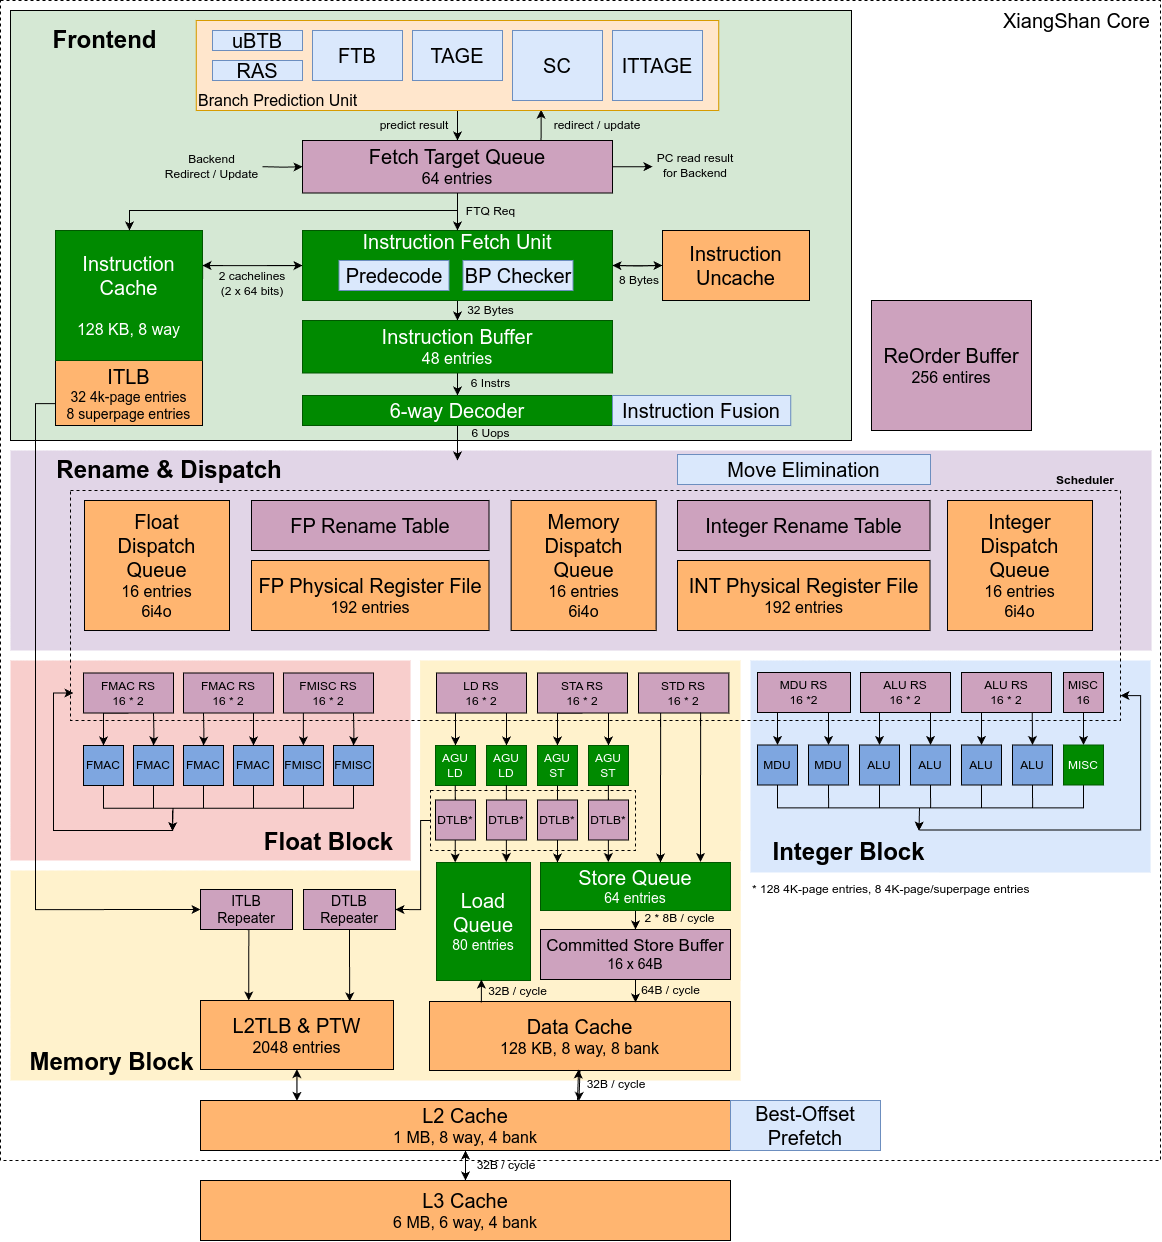
\includegraphics[scale=0.3]{xs-h-ext-priv.png}
    \caption{特权相关部件扩展涉及到的“南湖”的流水线}
    \label{fig:xs-h-ext-priv}
\end{figure}

\paragraph{特权控制}
该部分修改主要集中在控制状态寄存器执行单元中,包括特权级别的新增和控制状态寄存器的扩展。

\subparagraph{特权级别}
通过在硬件中添加虚拟位到原始的特权级别中,代表处理器是否开启了虚拟化,
用于区分虚拟机管理模式与虚拟监管模式、虚拟用户模式和普通用户模式。
同时,一级页表缓冲、地址翻译引擎、解码单元等模块需要当前的虚拟化模式信息,
所以需要在CSR执行单元的输出信号中添加虚拟化模式信号,将虚拟化模式信息传递到其他模块。

\subparagraph{控制状态寄存器}
需要添加的部分主要包括虚拟机管理模式的、虚拟监管模式的控制状态寄存器。
其中,虚拟管理模式下的相关CSR实现较为单一,仅需按照手册添加对应的功能:
包括配置处理器捕获敏感指令的能力,虚拟机管理模式的中断委托、使能、挂起等。
值得一提的是虚拟监管模式下的控制状态寄存器的读写处理。
根据当前特权级别中的虚拟位是否置起:控制状态寄存器的读写指令传入的寄存器地址可
以代表虚拟监管模式下的寄存器(例如stvec),
也可以代表对应的虚拟机管理模式下的寄存器(例如vstvec)。
所以需要使用当前特权级等信息对地址再映射。
此外,在虚拟机管理模式的CSR中,存在vsip和vsie这两个特殊的寄存器,
用于控制虚拟机中断的挂起和使能。
在实现方式上,不存在实际的物理寄存器,而是对mip和mie两个寄存器的切片映射。
例如,软件在读写,认为中断位为1、5、9位,但实际上是写入mip和mie的
2、6、10位,所以需要对读写数据进行特殊处理,根据读写寄存器是否是vsip
和vsie,来决定是否对数据进行移位操作。

\paragraph{特权指令}
特权指令均和第二阶段地址翻译相关,包括用于第二阶段页表的屏障指令HFENCE.VVMA/GVMA、
在未开启虚拟化模式时启用第二阶段地址翻译的访存指令HLV.width, HLVX.HU/WU, HSV.width。
作为特权指令,只能在非虚拟化模式下执行。
如果尝试在虚拟化模式下执行,则引发虚拟化指令异常,给控制流的异常向量信号的对应位赋值。
根据流水线由前至后的顺序,最先需要修改的是译码单元、派发、保留站部分。
这些部分因为Chisel高级语言的特性以及“香山”项目的良好基础架构,
仅需将指令添加到表格中,并指出所需派发到的保留站、功能单元的操作符等即可。
HFENCE.VVMA/GVMA指令需要交由屏障指令执行单元,访存相关指令交由内存访问流水线执行。
虚拟化访存指令是虚拟机管理系统访问虚拟机内存的手段,该类指令会启用两阶段地址翻译,
并且执行和虚拟机状态下一样的地址转换和类型检查。
该类指令主要在访存流水线中执行,并且执行的过程如表\ref{tab:h-ls}所示,
受多个控制状态寄存器影响。
除了对应的特权保护相关部分,需要在向一级页表缓冲发送地址翻译请求的时候,
指定是两阶段地址翻译,添加相关的控制状态寄存器的信息,例如ASID和VMID等。
虚拟化内存屏障指令则是复用了原有的内存屏障数据通路的状态机,
都是先等待写缓冲(Store Buffer)的清空,之后再向页表缓冲发送无效化的请求。
修改主要是对页表缓冲发送的无效化请求进行,在其中添加虚拟化内存屏障指令相关的字段。

\begin{table}
    \centering
    \caption{控制状态寄存器字段对虚拟化访存指令执行的影响}
    \begin{tabular}{cc}
        \toprule
        CSR字段        & 对虚拟化访存指令的影响      \\
        \midrule
        hstatus.hu   & 用户模式下能否执行虚拟化访存指令 \\
        hstatus.spvp & 控制虚拟化访存指令的执行特权级  \\
        sstatus.mxr  & 第二阶段的可执行权限页表是否可读 \\
        vstatus.mxr  & 第一阶段的可执行权限页表是否可读 \\
        \bottomrule
    \end{tabular}
    \label{tab:h-ls}
\end{table}

\section{内存管理单元设计扩展}
添加虚拟化扩展后的内存管理单元如图\ref{fig:after-mmu}所示,
主要的变化包括:添加第二阶段地址翻译单元、扩展一级页表缓存以支持两阶段地址翻译、
扩展二级页表缓存使其被两阶段页表共享、适配页目录翻译单元和叶表项翻译单元。
此外,该该部分还会分析Rocket Chip和CVA6,
目前两个实现了虚拟化扩展的开源RISC-V处理器的的虚拟内存管理单元和“香山”内存管理单元的优缺点。

\begin{figure}[htbp]
\centering
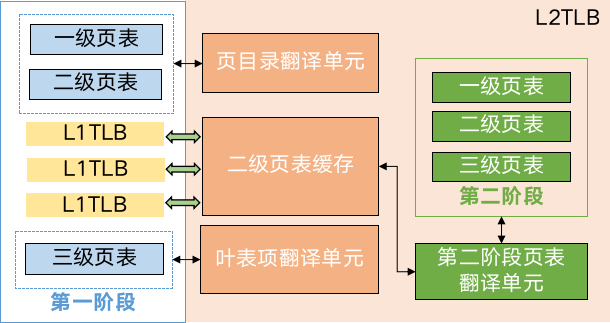
\includegraphics[scale=0.8]{after-mmu.png}
\caption{“香山”处理器添加虚拟化扩展后的内存管理单元}
\label{fig:after-mmu}
\end{figure}

\paragraph{第二阶段地址翻译单元}
该模块负责将虚拟机物理地址翻译成主机物理地址,需要多次访问内存解析页表。
实现方式采用朴素的阻塞状态机,一次仅处理一个请求。
但是对外暴露的端口采用的是Ready-Valid解耦形式的设计,
因此可以在不改变外部连接的情况下优化内部设计,以实现流水线或者并发。
在外部,和该模块直接相连的是二级页表缓存。
当向二级页表缓存查询第二阶段地址翻译不命中时,二级页表缓存会对该模块发起翻译请求。
翻译的结果会被缓存到二级页表缓存中。该模块相对于二级页表缓存,作为一个替换模块被使用。
因此,在初期使用阻塞的朴素实现,既可以观察二级页表缓存的缓存能力,也能够减少模块复杂度保证正确性。

\paragraph{二级页表缓存}
该模块是L2 TLB的中心,负责直接回复一级页表缓存的地址翻译请求。
在虚拟化扩展下,一级页表缓存会发送仅第一阶段、仅第二阶段和两阶段联合的三种类型的地址翻译请求。
但在原始架构下只实现了回复仅第一阶段的地址翻译的功能,
为了尽可能减少修改、同时尽可能快地回复三种类型的请求,通过在缓存条目中添加新的标志位区分页表的阶段。
具体而言,二级页表缓存中的所有缓存条目要么是仅第一阶段页表,要么是仅第二阶段页表,
和一级页表缓存条目完全不相同,不存在两阶段联合的缓存条目。
在这种设计下,可以快速的响应仅第一阶段的请求和仅第二阶段的请求。
对于两阶段联合的请求,则需要先向二级页表缓存发起第一阶段地址翻译请求,同时将请求缓存在寄存器。
得到第一阶段的翻译结果,即虚拟机物理地址后,再对二级页表缓存发起第二阶段地址翻译请求得到主机物理地址。
诚然,两阶段联合翻译时间是单阶段翻译时间的两倍,
但通过将二级页表缓存流水线化、使用不命中队列等方法,能够在一定程度上减少繁忙时期的查询开销。

虚拟化扩展下新增了HFENCE.VVMA和HFENCE.GVMA两条关于虚拟内存同步指令指令。
该指令用于在虚拟机管理模式下,同步内存中的两阶段的页表数据结构。
对于二级页表缓存,需要在执行指令时的将对应的,必须要无效化的条目无效化,
比如地址相同的或者是虚拟机编号(VMID)、进程编号(ASID)相同的条目。
仅无效化必要的条目可以称作精确无效化,但实现的复杂度较高。
也可以无效化全部条目保证以正确性和简便性,但是对效率较低。
另一方面,由于各级页表的不同数据分别存储在寄存器或者静态随机访问存储器(SRAM)
由于SRAM的同步读特性,精确无效化的实现难度相对寄存器言较高。
此外,各阶段各级页表的复用频率各不相同,需要在效率和实现复杂度中找到一个折中。
在目前的设计中,各阶段的各级页表缓存的有效位(valid)、全局位(global)和虚拟位(hypervisor)均使用寄存器实现。
因此均可简易地实现仅第一阶段或者第二阶段的页表无效化,
这种设计能够满足两种HFENCE指令的较低要求,即区分两阶段的页表。
进一步,对于VMID和ASID的精确无效化,仅在一级页表进行了实现。
因为其采用16项全相连的寄存器存储实现,可以较为快速地读取并计算需要无效化的条目。
而二级页表和三级页表的数据位均存储在SRAM中,难以实现快速的、简易的无效化。
最后,关于指定地址的精确无效化,只实现了第三级页表的大致的无效化。
则是使用指定地址的索引部分(index)查找存储器对应的条目,并将其无效化。
即不论标识部分(tag)是否相同,只要index相同则被无效化。
这种实现方式完全不需要读取SRAM,实现复杂度不高。
尽管会造成一定的性能损失,但是最多会将nWays(缓存路数)个不需要被无效化的条目无效,
是一个可接受的折中。

\paragraph{第一阶段地址翻译单元}
在虚拟化扩展下,第一阶段地址翻译单元仍然负责第一阶段的地址翻译。
最主要的修改是在每次访存前将客户机物理地址翻译成主机物理地址。
实现方式是通过增加自动机的状态,在发起访存请求前先对外发起第二阶段的地址翻译。
值得一提的是外界对第一阶段地址翻译单元发起的第二阶段地址翻译请求的回应方式。
如果直接发送到第二阶段地址翻译单元,无法充分利用二级页表缓存中的虚拟页条目。
因此请求会在仲裁后被先转发到二级页表缓存,如果不命中再由第二阶段地址翻译单元进行访存。
在这种方式下,一次命中可以减少3次内存访问,能够较为有效的提高翻译速度和二级页表缓存的利用率。

另一方面,第一阶段地址翻译单元由页目录和叶表项两个翻译单元组成,
分别负责第一阶段的前两级和最后一级的页表翻译。
两个模块虽然功能相似,实则具有不同的特点,在虚拟化扩展下也有不同的修改。
\subparagraph{页目录翻译单元}
主要的功能是作为二级页表缓存的替换单元,负责直接承接二级页表缓存的的不命中请求。
再根据请求的阶段和级数,转发给自己的自动机、叶表项翻译单元或者是进行第二级地址翻译。
因此实现上主要是体现一个灵活实现和功能接口丰富,接受所有可能的L2 TLB查询结果。
例如,在二级页表缓存的查询结果是第一阶段页表翻译直接命中页节点,但是第二阶段未命中。
此时将请求缓存,并发起第二阶段地址翻译,等待返回。
在二级页表查询结果是第一阶段页表翻译只命中了页目录,此时需要启动自己的自动机。
先发起第二阶翻译请求,将页目录的客户机物理地址翻译成主机物理地址;在根据返回结果判断权限、组合下一级页表的地址。
重复该过程直到找到叶表项的地址,之后把请求转发给叶表项翻译单元。
\subparagraph{叶表项翻译单元}
负责接收来自二级页表缓存和页目录翻译单元的叶表项翻译请求。
请求的频率必然高于页目录翻译单元,因此在实现上主要追求高并发和快速。
优化的切入点在于叶表项总是连续的,可以使用猝发访存,一次获取多个相邻的叶表项。
在硬件实现上,存在多个缓存槽,因此叶表项翻译单元可以非阻塞的接收多个请求。
每此接收新请求,分配缓存槽的时候,会根据请求的虚拟机物理地址判断是是否位于同一缓存行,
能否在同一个猝发访存中得到结果。如果可以,新请求会使用等待槽编号记录旧请求的缓存槽编号。
当访存返回时,对所有等待槽编号与该访存的缓存槽编号相同的缓存槽的状态进行转换。
代表访存结果已经返回,之后由出队逻辑将所有已完成的缓存槽逐个出队。
然而,在虚拟化扩展下,访存返回的仅仅是虚拟机物理地址,
还需要再经过一次第二阶段地址翻译将其翻译成主机物理地址。
现阶段的实现是使用自动机第二阶段翻译请求向外发送,
该请求会与页目录翻译单元的第二阶段请求进行仲裁后会被发送到二级页表缓存查询。
叶表项翻译单元不需要理解外界如何处理其第二阶段地址翻译请求,只需要等待翻译结果并返回即可。
尽管这是一个不太有效率的做法,但是没有破坏原本的第一阶段叶表项的高吞吐量。

\paragraph{一级页表缓存}
一级页表缓存作为分布式的小容量全相连页表缓存,
分布式地布线在取指单元(IFU)和访存单元(Memory Block),能够减少时序压力。
主要负责通过一个时钟周期的时间,快速地将虚拟机虚拟地址转换为主机物理地址。
为了在支持快速地两阶段地址翻译的同时,兼容仅第一阶段的地址翻译,
需要在缓存条目中添加虚拟化位和虚拟机标识。
此外,一个缓存条目还存储了多个权限阶段等信息相同的有效的物理地址。
即可以根据虚拟地址的低位标识(tag)来索引不同的物理地址。
该优化的想法来源于连续的虚拟页的权限和异常信息可能具有局部性,
而且来自二级页表缓存的充填数据是以缓存块的形式返回多个翻译结果。
实现则是通过使用一组寄存器,按照虚拟地址的低3位标识存储物理地址的低3位标识。
较少的组数,可以保证布线的负担不会太大,对于特殊情况的优化效果也是明显的。

虚拟化扩展在异常方面也需要一级页表缓存提供额外的支持。
即虚拟机缺页异常,表示在进行第二阶段地址翻译是触发了缺页。
在实现方面,一级页表缓存仅保存是否发生了相关异常,而异常所对应的虚拟机物理地址,由于容量原因则不保存在数据表项中。
需要在响应请求时判断:如果命中的页表条目发生了虚拟机缺页异常,
则返回不命中,同时向二级页表缓发起翻译请求,直到返回虚拟机物理地址后,一级页表缓存才会响应命中。
鉴于虚拟机缺页异常发生频率较低,这种以时间换面积开销的解决方案是可接受的。

\section{设计扩展正确性评测}
为了验证虚拟化扩展实现的正确性,
本文使用riscv-hyp-test\cite{itco2022rocket}进行验证。
这是一个开源的,针对RISC-V的虚拟化扩展的测试,是一个小型的裸机程序。
最初是是Rocket Chip在开发虚拟化时编写的,用于加速开发的简易测试。
如表\ref{tab:hyp-test}所示,
hyp-test包括特权指令、虚拟内存、异常中断三个方面,每个方面都有若干个小测试。

\begin{table}
    \centering
    \caption{riscv-hyp-test的测试和功能}
    \begin{tabular}{ccc}
        \toprule
        类别   & 基准测试                          & 测试目标             \\
        \midrule
        特权指令 & wfi exception tests           & VS和HS下执行wfi指令    \\
        特权指令 & hfence test                   & HS的页表同步指令        \\
        特权指令 & virtual instruction           & VS下执行hyper特权指令   \\
        虚拟内存 & two stage translation         & VS下通过两级页表翻译访问内存  \\
        虚拟内存 & second stage only translation & HS下仅第二级页表翻译访问内存  \\
        虚拟内存 & m and hs using vs access      & HS下通过两级页表翻译访问内存  \\
        异常中断 & interrupt tests               & HS下挂起虚拟机中断       \\
        异常中断 & check xip regs                & HS下中断委托、挂起寄存器    \\
        异常中断 & tinst tests                   & HS和VS异常需写入特定的CSR \\
        \bottomrule
    \end{tabular}
    \label{tab:hyp-test}
\end{table}

测试的运行环境是开源的逻辑软件仿真工具verilator。
由于该测试程序不需要任何引导程序或者操作系统,
把测试程序的二进制文件放入仿真内存的处理器复位时跳转的地址,即可正常执行。
采用软件逻辑仿真的是因为是测试程序足够小,能够在几分钟内快速的完成。
此外,逻辑仿真软件能够获取波形文件,对硬件调试有巨大的帮助。
然而,完全运行测试仍然需要数万个时钟周期,无法精确地定位出错现场。
因此还使用了差分测试的方法来快速地定位错误时刻。
通过使用RISC-V处理器模拟器NEMU,一个软件实现的处理器金标准。
在每条指令执行的时候,对比“香山”和金标准的所有架构处理器。
可以将错误发生现场缩短在一条指令的执行周期内。
在以上工具的帮助下,通过了每个方面的测试,运行结果如图\ref{fig:hyp-test}所示。

\begin{figure}[htbp]
    \centering
    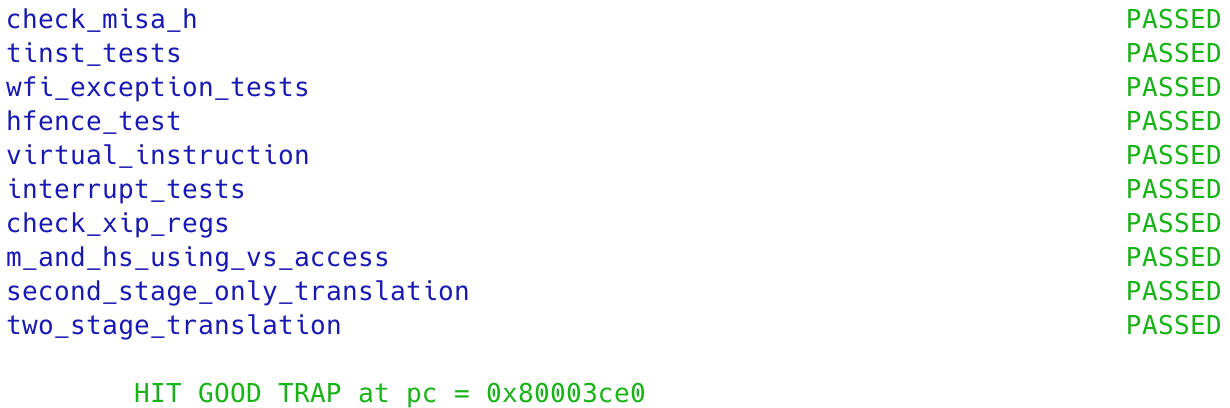
\includegraphics[scale=0.45]{hyp-test.png}
    \caption{在差分测试框架中运行hyp-test结果}
    \label{fig:hyp-test}
\end{figure}

\section{本章小结}
本章介绍“香山”处理器的“南湖”架构的虚拟化扩展的硬件实现。
虚拟化扩展的修改,可以分为特权相关部件和内存管理单元两部分。
在完成了硬件扩展后,使用一个专用于RISC-V虚拟化扩展的小型裸机程序测试,测试功能的正确性。
\chapter{系统软件下的初步评测}

在完成基本的功能正确性评估后,本文尝试启动Linux操作系统,这是使用KVM启动虚拟机的前提。
本章讲述启动操作系统时对软件进行的适配,以及软硬件联合调试是遇到的困难及解决方案。
同时还对主机性能进行了相关评测,作为虚拟机性能评测的基准线。

\section{操作系统的适配与启动}
关于目标适配的虚拟化软件Linux KVM,是一个开源的Type2虚拟机管理系统。
在RISC-V架构方面,已经存在初步适配后的软件——kvm-riscv\cite{github:riscv-kvm},
该项目主要包括启动KVM选项并适配RISC-V架构后的Linux源码及配置、包括kvmtool的根文件系统。
该套完整系统软件可以直接在RISC-V处理器模拟器(qemu、spike)中运行。

特别是kvmtool,这是一个Linux的用户态程序。
通过在命令行中执行该工具,可以直接使用KVM启动虚拟机。
为了能够在命令行中使用该工具,需要手动编译该软件并将其放入根文件系统中,
考虑到根文件系统应该尽可能小,尽可能简便,
根文件系统中无需包含动态链接的可执行程序的系统库,例如libc和libm。
为此,kvmtool需要静态编译,包括其依赖库libfdt,也需要静态编译后,一起链接到kvmtool中。

本文计划在FPGA中部署硬件直接启动Linux和KVM,通过观察串口输出判断是否正常运行。
因为完成操作系统的启动至少需要3亿以上的周期数,
逻辑软件仿真的速度太慢,需要花费数天的时间才能完成。
因此,需要让系统软件对FPGA平台进行一定的适配:
编写对应平台专用设备树,根据FPGA使用的外设开启相应驱动。

完成软件适配之后,需要在FPGA上启动进行软硬件联合调试。
但是在尝试启动Linux时遇到了难以调试的问题:
Linux的输出如图\ref{fig:console-block}所示,
在输出hvc0 console的初始化信息后,就不再有任何输出。
由于在FPGA运行无法获取波形图,难以观察电路内部的情况。
此时离上电复位也经过了数百万个周期,即使使用逻辑仿真也需要极长的时间才能运行到出错点。

\begin{figure}[htbp]
    \centering
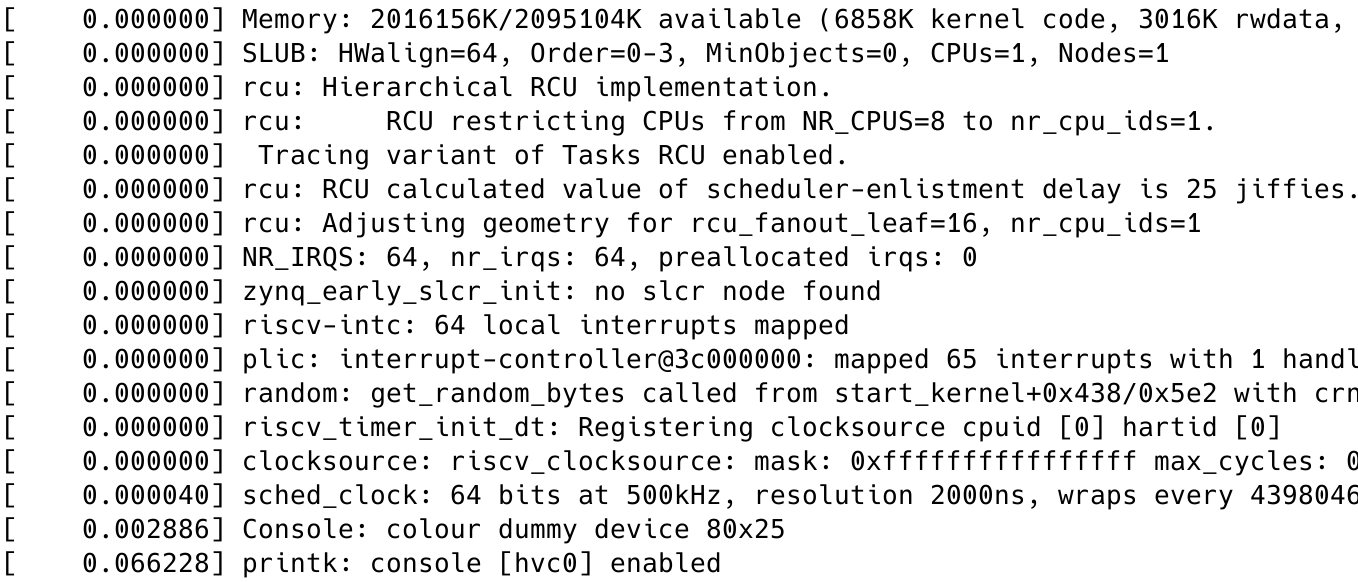
\includegraphics[scale=0.4]{hvc.png}
    \caption{虚拟化扩展后的“香山”启动Linux的串口输出}
    \label{fig:console-block}
\end{figure}

为了能够快速仿真到出错点,并且使用逻辑仿真软件生成波形的能力观察电路内部细节,
本文使用REMU\cite{iccd2023remu}——基于FPGA的加速仿真平台,进行调试。
平台的实物图如\ref{fig:remu-card}所示。
通过使用REMU,可以在FPGA中快速地将Linux启动到任意时刻,然后使用ctrl-c中断现场,
并将此时硬件内部所有寄存器和存储器通过检查点的方式保存。
检查点数据通过DMA从FPGA发送到x86主机后,
可以被逻辑仿真软件工具重放,即可快速地得到数百万周期后的波形。



\begin{figure}[htbp]
    \centering
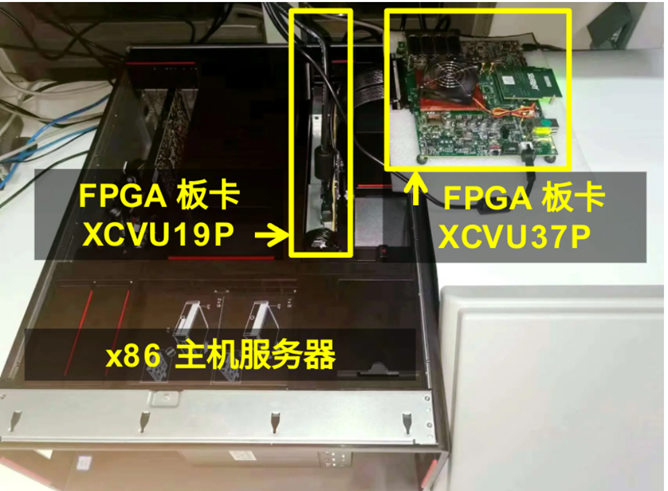
\includegraphics[scale=0.7]{remu-card.png}
    \caption{REMU平台硬件实体}
    \label{fig:remu-card}
\end{figure}

通过观察如图\ref{fig:console-block-wave}所示的REMU重放波形,
可以清楚地观察到处理器在某一时刻后没有提交任何指令,也没有对外发起任何访存请求。
造成这种现象的一般原因是某一级流水线的自动机设计缺陷:
某种特殊情况使得状态机停滞在某一状态,无法进行状态切换,导致整个处理器停滞。
经过细致的波形分析即可发现,是指令缓存的状态机设计的缺陷。
在某种特殊的不命中的情况下,既不对外发起访存请求,也不使用内部缓存块数据返回。
在REMU的帮助下,找到了错误的代码进行修改后,Linux能够正常启动。

\begin{figure}[htbp]
    \centering
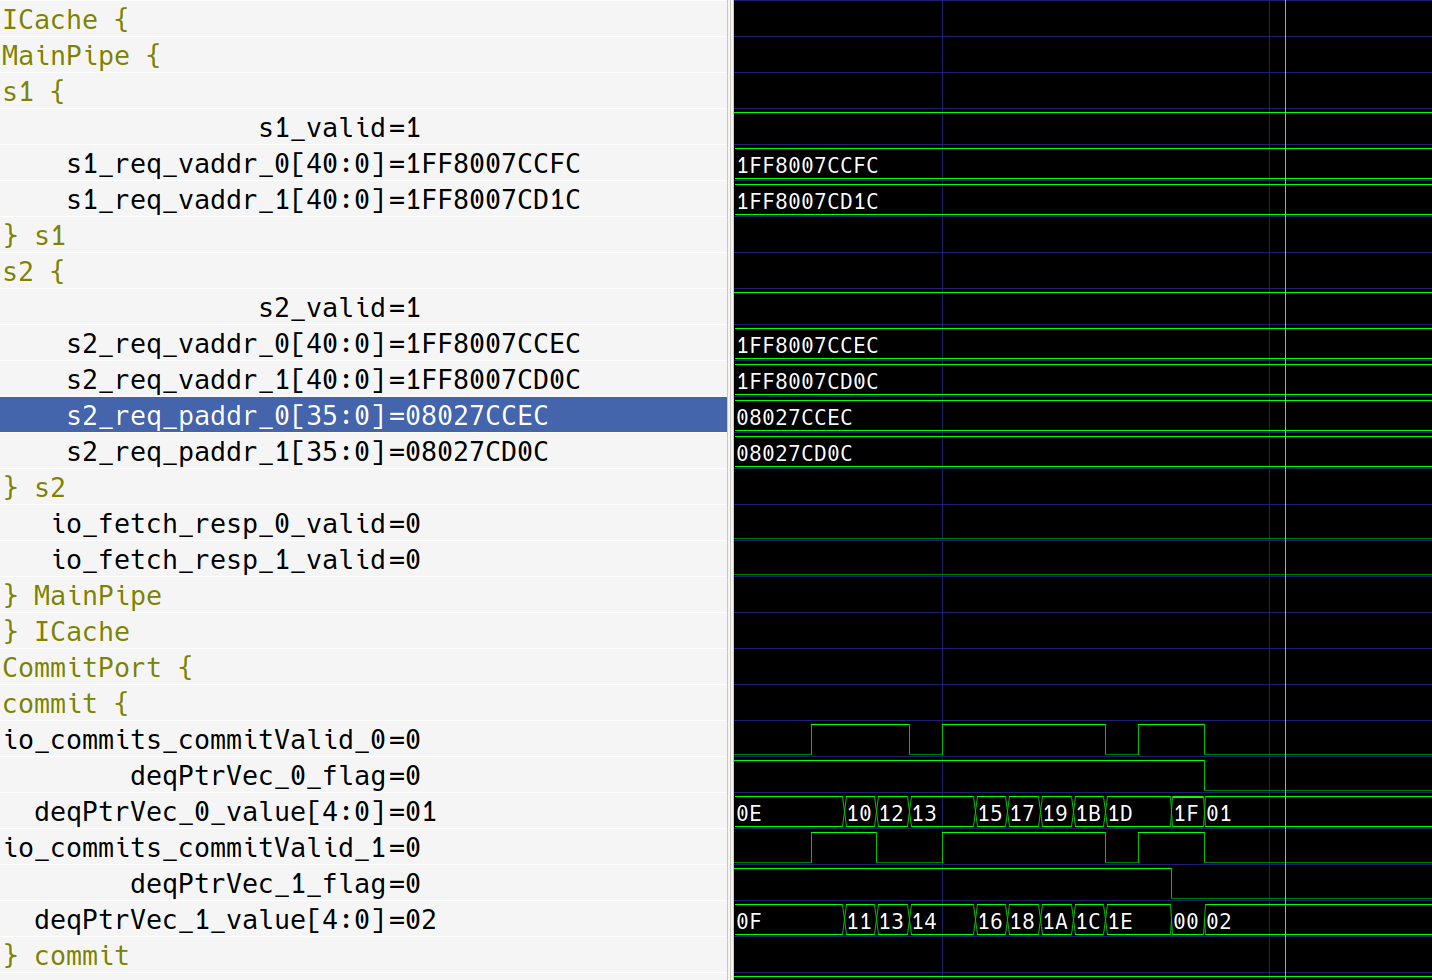
\includegraphics[scale=0.35]{icache-block.png}
    \caption{REMU重放的Linux启动波形}
    \label{fig:console-block-wave}
\end{figure}

\section{操作系统下的性能评测}
在多年发展下,虚拟化评测已成为一个研究良好的领域,开发了许多评估各种虚拟化平台性能的基准方法。
根据粒度将现有的基准大致分为微观基准和宏观基准。
宏观基准评估实际应用程序在松散定义的条件下的整体性能,如lmbench、SPEC CPU 2006等。
微观基准测试衡量的是在定义良好的条件下单个原始操作的性能。
但是不论是宏观还是微观,其中一个重要的基准线便是主机性能,即未开启虚拟化下运行基准测试的性能。
该阶段已经完成Linux操作系统的启动,在评估虚拟化性能前,可以先对主机性能进行简单评测。
于是,同样在FPGA平台中,使用虚拟化扩展的“香山”处理器,启动Linux。
在Linux中,通过命令行运行CoreMark和Dhrystone基准测试,运行输出如图\ref{fig:coremark}和\ref{fig:dry}所示。
同时,作为对比也使用了未添加虚拟化扩展的“香山”处理器进行,对比结果如图\ref{tab:perf}所示。
根据测试结果可以看出,虚拟化扩展的添加,对主机性能影响并不大,保持了原有的高性能乱序核的特点。

\begin{table}
    \centering
    \caption{原始“香山”与虚拟化扩展后的“香山”的基准测试}
    \begin{tabular}{ccc}
        \toprule
        基准测试名称   & 原始“香山”跑分 & 虚拟化扩展后“香山”跑分 \\
        \midrule
        CoreMark & 191.22   & 190.7        \\
Dhrystone & 81433   & 77680        \\
        \bottomrule
    \end{tabular}
    \label{tab:perf}
\end{table}



\begin{figure}[htbp]
    \centering
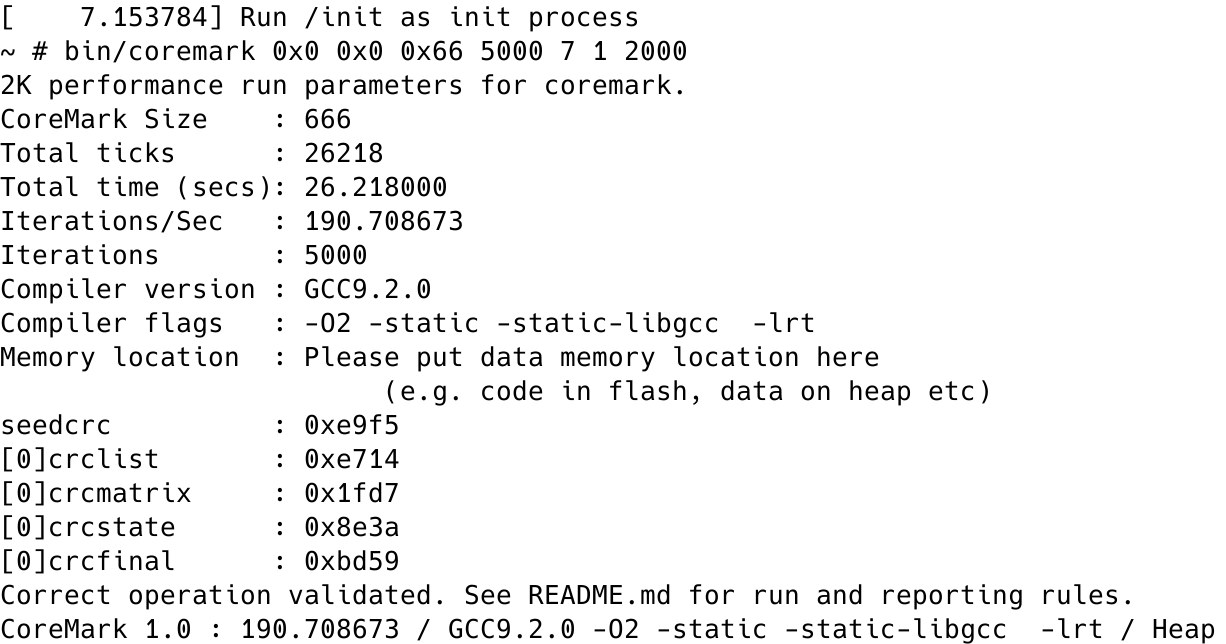
\includegraphics[scale=0.4]{coremark.png}
\caption{虚拟化扩展后的“香山”迭代5000次运行CoreMark}
\label{fig:coremark}
\end{figure}

\begin{figure}[htbp]
    \centering
    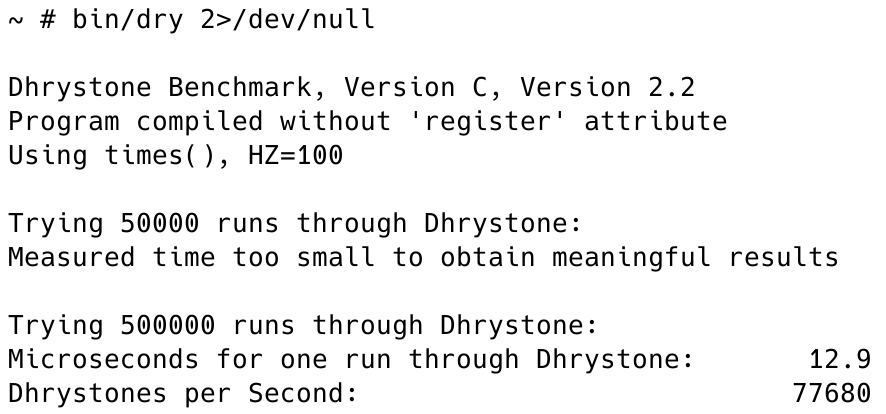
\includegraphics[scale=0.4]{h-ext-dry.png}
    \caption{虚拟化扩展后的“香山”迭代500000次运行Dhrystone}
    \label{fig:dry}
\end{figure}



\chapter{虚拟机管理系统的调试}
通过对系统软件的修改移植,现阶段可以在添加虚拟化扩展的“香山”处理器中启动操作系统,
运行主机级别用户态程序,并对主机性能进行了简单的评测。
下一步需要运行虚拟机,并尝试在虚拟机中运行相同的用户态程序,以评测虚拟化性能。
本章描述在使用虚拟化扩展的“香山”运行KVM,其中遇到的难以调试的错误以及对调试方案的探索。

\section{虚拟机启动的现象}
在命令行工具中通过kvmtool工具,尝试启动虚拟机。
但是串口输出如图\ref{fig:kvm-run}所示,没有进一步虚拟机Linux启动的输出。

\begin{figure}[htbp]
    \centering
    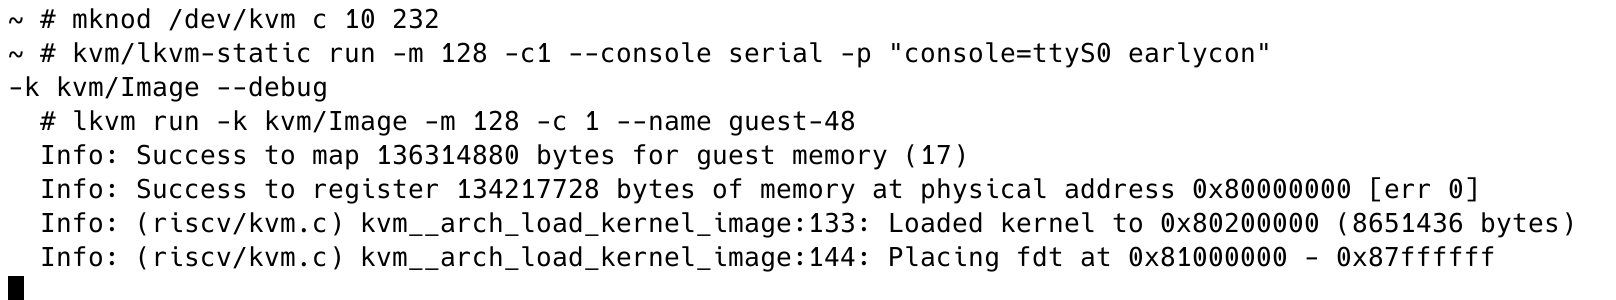
\includegraphics[scale=0.35]{kvm-run.png}
    \caption{使用kvmtool启动虚拟机的串口输出}
    \label{fig:kvm-run}
\end{figure}

为了观察电路内部状态,使用REMU重放此刻的波形。
波形如图\ref{fig:kvm-wave}所示,可以得出如下所示的现象:

\begin{itemize}
    \item 指令提交没有停止,在正常流动
    \item 指令的虚地址位于\verb|1FF_800X_XXXX|区域,物理地址位于\verb|802X_XXXX|区域
    \item 处理器目前运行在虚拟机监管模式,尚未开启虚拟位
    \item 控制状态寄存器satp.mode值为8,代表第一阶段地址翻译正常开启
\end{itemize}

尽管可以从波形中获取更多的体系结构、甚至是微架构信息,但是对调试帮助甚微。
因为调试还需了解此刻正确的体系结构信息,通过比对正确和已有的体系结构信息,才能进一步反推出错原因。
换言之,只有找出体系结构信息出错的现场、甚至是第一现场,才能帮助处理器调试。
但此时距离处理器上电复位已经运行了49亿以上的时钟周期,
处理器的内部状态十分复杂,难以确定此刻正确的体系结构信息。
一方面,无法知道处理器在运行软件的哪一部分,
可能是系统软件,也可能是被加载到内存中的应用程序。
因为虚拟地址的使用,导致加载地址是可浮动的,这会将极大的增加软硬件联合调试的难度。
另一方面,纵使知道了“香山”处理器在执行当前系统的软件的哪一部分,也很难获取此时处理器内正确的体系结构信息。
尽管可以使用其他的处理器,或者是模拟器运行相同的系统软件,并停止在该部分。
但是执行中所需的外设输入,访存延时等各种不确定信息需要被精确重放在其他的处理器中,
才有可能保证两个处理器对同一系统软件的执行路径是相同的,从而得到可用的、正确的的体系结构信息。
综上所述,为了调试错误,当务之急是找到一种既能精确定位错误现场,又能通过仿真快速迭代的调试手段。

\begin{figure}[htbp]
    \centering
    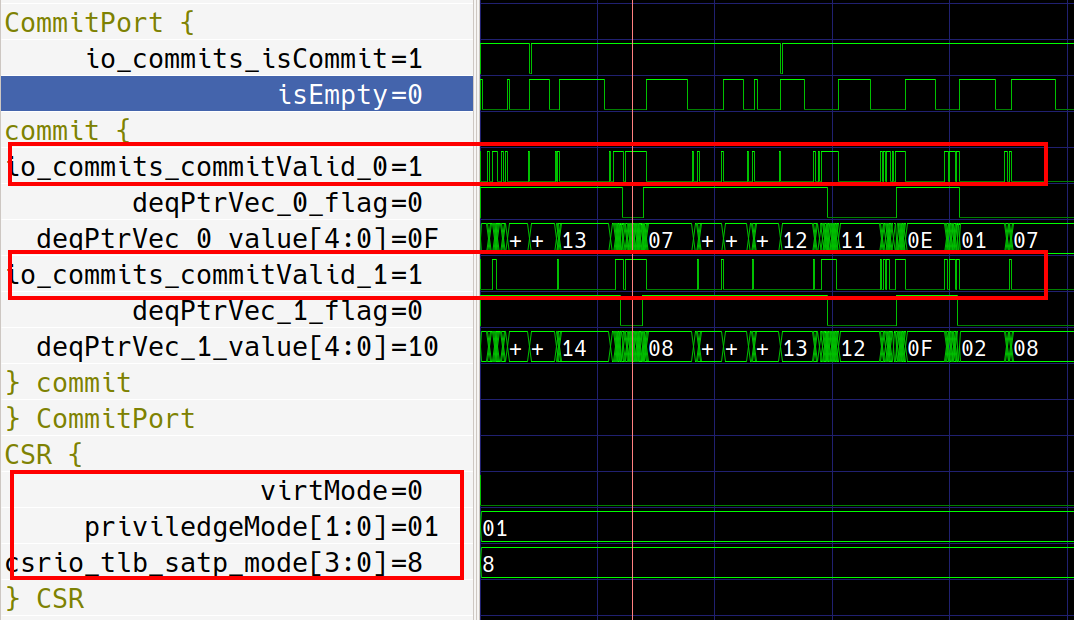
\includegraphics[scale=0.5]{kvm-wave.png}
    \caption{使用kvmtool启动虚拟机的串口输出}
    \label{fig:kvm-wave}
\end{figure}

\section{现有调试手段的限制}
现阶段,“香山”处理器官方调试方法依然是纯软件仿真和差分测试。
通过实时比对“香山”处理器和处理器模拟器NEMU的体系结构信息,
并在一些关键的时刻,例如中断、外设输入等,让“香山”指导模拟器的执行路径。
从而保证了在任意时刻,“香山”处理器的体系结构信息是正确的。
一旦在体系结构信息层面出现微小的错误,差分测试框架会立刻停止仿真并汇报错误。
然而,逻辑仿真软件的速度是不可接受的。
为了调试上述错误,尝试使用差分测试框架进行逻辑仿真。
结果表示,上电复位开始进行逻辑仿真,花费两天时间仍然无法完成Linux的启动。
由此可见,尽管软件仿真能够精确的定位错误现场,速度是最主要的限制。

另一方面,基于FPGA的加速仿真框架REMU,
虽然可以使用FPGA加快仿真的速度,并在逻辑仿真软件中精确地重放波形。
但是仅作为一个仿真框架,无法提取体系结构信息、
实时和正确的体系结构信息进行比对,导致难以精确地定位错误现场。
对REMU而言,最主要的限制在于其灵活性,即使用方式。
在现阶段的功能下,只有在部分特殊的情况下,
即可以从波形明显看出出错现场的时刻,波形重放工具才能够独立的完成错误调试的任务。
在大部分情况下,包括目前遇到的问题,尚不足以解决。
为了调试KVM运行卡住的原因,仅存在重放波形唯一的使用方法。
但通过波形重放,无法明显的看出具体问题。
不同于单纯的硬件卡死卡住,此时指令一直流动,但不知道处理器在运行软件的哪一部分。
一旦脱离了体系结构信息,处理器调试会变得毫无根据。
为此REMU在处理器调试方面,急需一套完整能够提取体系结构信息的基础设施。

\section{潜在调试方案的探索}

\paragraph{逻辑仿真软件}
上述提到软件仿真的主要限制是速度,从上电复位开始仿真到操作系统启动所需的时间很长。
那可以考虑从操作系统启动之后开始仿真,跳过已经能够正确运行的操作系统启动部分。
“香山”官方的配套基础设施也有类似的支持。
他们为NEMU,“香山”专用的处理器模拟器,添加了生成检查点的功能。
NEMU可以在运行任意负载的任意时刻停下,将此刻的体系结构信息保存成检查点。
这里描述的检查点,是此时NEMU执行至此的内存布局。
同时还在内存指定的地方,存储所有的体系结构寄存器信息。
在“香山”处理器进行逻辑仿真的时刻,会先执行一段汇编。
通过访存指令,从内存指定的地方加载所有的寄存器的数值到对应的体系结构寄存器中。
之后使用跳转执行继续检查点的下一条指令。

换言之,使用“香山”官方提供的检查点方法,
能够把启动完操作系统的处理器的体系结构信息放入“香山”后,再启动仿真。
但是对于微架构寄存器则无能为力,
因为既不存在、也没必要存在一个和“香山”微架构一模一样的模拟器。
尽管这种方法可以复现部分错误,
但是对于类似数据缓存、页表缓存、页表翻译单元等没有任何体系结构信息的单元,
无法复现错误的概率也很大。
缓存单元的错误很可能在上电复位之后会被隐藏,正是在持续运行中才有可能暴露。
尽管如此,不论是否能发现错误,本文中依然尝试了该方法进行处理器的调试。
然而在系统软件的适配中遇到了问题,由于时间限制,尚未完成调试。
关于系统软件的问题,由于NEMU和“香山”的SoC在启动时暂时不支持外存,所以根文件系统必须要和内核镜像打包在一起。
然而尝试使用NEMU单独启动操作系统之后,仍无法完成init进程的启动进入Shell,如图\ref{fig:init-block}所示。
为了解决该问题,下一步需要使用QEMU和gdb进行联合调试,解决软件中潜在的问题。

\begin{figure}[htbp]
    \centering
    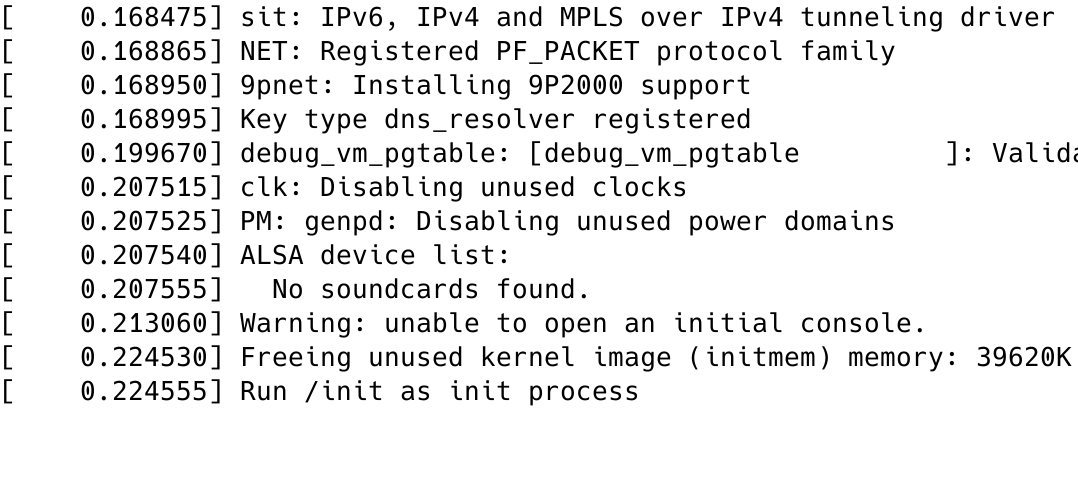
\includegraphics[scale=0.5]{init-block.png}
    \caption{NEMU启动Linux时无法完成init进程的加载}
    \label{fig:init-block}
\end{figure}

\paragraph{FPGA平台}
关于FPGA硬件加速仿真平台REMU,目前的检查点和波形重放功能十分单一,支持的逻辑仿真软件只有iverilog。
纵使想要使用REMU生成的检查点,重放到差分测试的仿真框架中这也是做不到的。
差分测试的仿真框架目前仅支持verilator和Synopsys VCS两种逻辑仿真工具。
分别是目前开源社区和商业界最高效的仿真工具,可配置程度高,仿真激励部分使用C++语言编写。
相比之下iverilog是更偏向教学与学术研究的工具,上手难度较低,
仿真激励部分使用verilog语言编写;相对的,在仿真速度和可配置程度上无法和verilator相比。
为了能让REMU的检查点发挥更大作用,支持verilator是一个必经之路。

为了将检查点数据放入逻辑仿真软件中,
REMU使用了verilog的语言规范中定义的编程接口:Verilog Procedural Interface(VPI)。
VPI作为一个语言规范,在iverilog和verilator中均有不同程度的部分实现。
然而对于重放检查点而言,仅仅需要满足向物理寄存器写入数据这一需求。
iverilog和verilator均存在对应的VPI实现,因此存在部分可复用的代码。
所需做的是使用C++编写verilator的仿真激励,修改部分verilator和iverilog不兼容的部分。
尽管目前已经能够使用verilator重放REMU检查点,但是在实用化上还远远不够。
后续还需要对接差分测试的仿真框架与目前已有的verilator仿真框架。
包括把检查点的数据放入模拟器NEMU在差分测试的仿真激励脚本中添加VPI的相关代码等。
该部分虽然仅只是作为工程实现,没有太多的设计创新的部分。
但是为REMU丰富了使用的方法,为后续REMU的差分测试硬件化打下基础。

仅仅实现逻辑仿真软件重放检查点数据是不够的,REMU需要更为精确的定位错误现场的方法。
可以考虑将差分测试的部分逻辑固化在FPGA中,同时利用FPGA的快速和差分测试的精准。
具体的固化实现是将FPGA中对应各种架构寄存器的物理寄存器、差分测试的使能信号等,
通过硬连线拉出到顶层,每周期进行采样。
对于需要比对的数据,则以DMA的形式从FPGA发送相连的x86主机中,再与模拟器进行比对。
这种差分测试硬件化的想法尽管在REMU平台发布时已经提出,
并对NutShell——国科大学生设计的顺序核,进行了适配,
但是对于“香山”处理器还未达到可用的地步,还需要进一步修改。
除了可用性的适配之外,还需要考虑的一部分则是处理速度,
需要完全精确地硬化差分测试中,FPGA每周期需要采样大量数据进行DMA,
DMA的传输速度和软件处理数据的速度会逐渐成为FPGA加速仿真的瓶颈。
因此需要精心设计传输数据的格式,或者降低比对的频率,如多条指令提交后才进行一次比对。
其本质都是减少数据传输量,降低DMA和软件侧的负荷。
该部分的工作也因为时间限制尚未完成,会在今后成为研究方向。
\backmatter
% !Mode:: "TeX:UTF-8" 
\begin{conclusions}

本文围绕着为RISC-V开源处理器"香山"的南湖架构添加虚拟化扩展,
讲述了对虚拟化微架构、系统软件和调试工具三个方面的研究。
第一,在虚拟化微架构上,扩展了“香山”特权控制和虚拟内存两部分的设计,从而实现了虚拟化扩展。
特别是虚拟内部分,通过添加第二阶段地址翻译单元、复用二级页表缓存等能够加快页表翻译的微架构。
第二,在添加虚拟化扩展的“香山”上尝试启动Linux和虚拟机管理系统KVM。
在FPGA加速仿真工具REMU的调试帮助下,Linux能够顺利启动。
但是在启动KVM虚拟机时,由于硬件设计还是存在尚未发掘的错误而失败。
第三,为了找出错误,尝试了基于纯软件逻辑仿真的差分测试以及基于FPGA的仿真加速平台等调试工具。
但由于软硬件联合调试的复杂性以及现有调试工具的能力限制,问题未能解决。
因此,对扩展现有调试工具的能力方面进行了探索:
基于纯软件仿真的差分测试工具,可以联合使用体系结构信息检查点,跳过不必要的操作系统仿真步骤。
基于FPGA的仿真加速工具,可以在差分测试框架中重放微架构检查点,或者是将差分测试硬件化在FPGA中。

\end{conclusions}
   % 结论
\bibliographystyle{gbt7714-numerical}
% \bibliographystyle{hitszthesis} % 深圳校区的同学请使用 hitszthesis 文献样式
%\bibliographystyle{hithesis} %理论上2020最新要求文献样式GB/T 7714—2015,但若院系要求文献英文作者不全大写,可改用hithesis文献样式
%%%%%%%%%%%%%%%%%%%%%%%%%%%%%%%%%%%%%%%%%%%%%%%%%%%%%%%%%%%%%%%%%%%%%%%%%%%%%%%%
%-- 注意:以下本硕博、博后书序不一致 --%
%%%%%%%%%%%%%%%%%%%%%%%%%%%%%%%%%%%%%%%%%%%%%%%%%%%%%%%%%%%%%%%%%%%%%%%%%%%%%%%%
% 本科书序(哈尔滨、深圳校区)
%%%%%%%%%%%%%%%%%%%%%%%%%%%%%%%%%%%%%%%%%%%%%%%%%%%%%%%%%%%%%%%%%%%%%%%%%%%%%%%%
\bibliography{reference} % 参考文献
\authorization %授权
% \authorization[scan.pdf] %添加扫描页的命令,与上互斥
% !TEX root = ../main.tex

% 致谢
\begin{acknowledgements}
衷心感谢导师~XXX~教授对本人的精心指导。他的言传身教将使我终生受益。

……

感谢哈深\LaTeX{}论文模板\hitszthesis\ !

\end{acknowledgements}
 %致谢
\begin{appendix}%附录
    % !TEX root = ../main.tex

% 附录1
\chapter{外文资料翻译}
% 设置附录页码从1开始编号
% \SetPageNumberingFromOne

\title{英文资料的中文标题}

{\heiti 摘要:} 本章为外文资料翻译内容。如果有摘要可以直接写上来,这部分好像没有
明确的规定。

\section{单目标规划}
北冥有鱼,其名为鲲。鲲之大,不知其几千里也。化而为鸟,其名为鹏。鹏之背,不知其几
千里也。怒而飞,其翼若垂天之云。是鸟也,海运则将徙于南冥。南冥者,天池也。
\begin{equation}\tag*{(123)}
 p(y|\mathbf{x}) = \frac{p(\mathbf{x},y)}{p(\mathbf{x})}=
\frac{p(\mathbf{x}|y)p(y)}{p(\mathbf{x})}
\end{equation}

吾生也有涯,而知也无涯。以有涯随无涯,殆已!已而为知者,殆而已矣!为善无近名,为
恶无近刑,缘督以为经,可以保身,可以全生,可以养亲,可以尽年。

\subsection{线性规划}
庖丁为文惠君解牛,手之所触,肩之所倚,足之所履,膝之所倚,砉然响然,奏刀騞然,莫
不中音,合于桑林之舞,乃中经首之会。
\begin{table}[ht]
  \centering
  \wuhao
  \caption*{表~1\hskip1em 这是手动编号但不出现在索引中的一个表格例子}
  \label{tab:badtabular3}
  \begin{tabular}[c]{|m{1.5cm}|c|c|c|c|c|c|}\hline
    \multicolumn{2}{|c|}{Network Topology} & \# of nodes &
    \multicolumn{3}{c|}{\# of clients} & Server \\\hline
    GT-ITM & Waxman Transit-Stub & 600 &
    \multirow{2}{2em}{2\%}&
    \multirow{2}{2em}{10\%}&
    \multirow{2}{2em}{50\%}&
    \multirow{2}{1.2in}{Max. Connectivity}\\\cline{1-3}
    \multicolumn{2}{|c|}{Inet-2.1} & 6000 & & & &\\\hline
    & \multicolumn{2}{c|}{ABCDEF} &\multicolumn{4}{c|}{} \\\hline
\end{tabular}
\end{table}

文惠君曰:“嘻,善哉!技盖至此乎?”庖丁释刀对曰:“臣之所好者道也,进乎技矣。始臣之
解牛之时,所见无非全牛者;三年之后,未尝见全牛也;方今之时,臣以神遇而不以目视,
官知止而神欲行。依乎天理,批大郤,导大窾,因其固然。技经肯綮之未尝,而况大坬乎!
良庖岁更刀,割也;族庖月更刀,折也;今臣之刀十九年矣,所解数千牛矣,而刀刃若新发
于硎。彼节者有间而刀刃者无厚,以无厚入有间,恢恢乎其于游刃必有余地矣。是以十九年
而刀刃若新发于硎。虽然,每至于族,吾见其难为,怵然为戒,视为止,行为迟,动刀甚微,
謋然已解,如土委地。提刀而立,为之而四顾,为之踌躇满志,善刀而藏之。”

文惠君曰:“善哉!吾闻庖丁之言,得养生焉。”


\subsection{非线性规划}
孔子与柳下季为友,柳下季之弟名曰盗跖。盗跖从卒九千人,横行天下,侵暴诸侯。穴室枢
户,驱人牛马,取人妇女。贪得忘亲,不顾父母兄弟,不祭先祖。所过之邑,大国守城,小
国入保,万民苦之。孔子谓柳下季曰:“夫为人父者,必能诏其子;为人兄者,必能教其弟。
若父不能诏其子,兄不能教其弟,则无贵父子兄弟之亲矣。今先生,世之才士也,弟为盗
跖,为天下害,而弗能教也,丘窃为先生羞之。丘请为先生往说之。”

柳下季曰:“先生言为人父者必能诏其子,为人兄者必能教其弟,若子不听父之诏,弟不受
兄之教,虽今先生之辩,将奈之何哉?且跖之为人也,心如涌泉,意如飘风,强足以距敌,
辩足以饰非。顺其心则喜,逆其心则怒,易辱人以言。先生必无往。”

孔子不听,颜回为驭,子贡为右,往见盗跖。

\subsection{整数规划}
盗跖乃方休卒徒大山之阳,脍人肝而餔之。孔子下车而前,见谒者曰:“鲁人孔丘,闻将军
高义,敬再拜谒者。”谒者入通。盗跖闻之大怒,目如明星,发上指冠,曰:“此夫鲁国之
巧伪人孔丘非邪?为我告之:尔作言造语,妄称文、武,冠枝木之冠,带死牛之胁,多辞缪
说,不耕而食,不织而衣,摇唇鼓舌,擅生是非,以迷天下之主,使天下学士不反其本,妄
作孝弟,而侥幸于封侯富贵者也。子之罪大极重,疾走归!不然,我将以子肝益昼餔之膳。”%本科生翻译论文
\end{appendix}
%%%%%%%%%%%%%%%%%%%%%%%%%%%%%%%%%%%%%%%%%%%%%%%%%%%%%%%%%%%%%%%%%%%%%%%%%%%%%%%%
% 本科书序(威海校区)
%%%%%%%%%%%%%%%%%%%%%%%%%%%%%%%%%%%%%%%%%%%%%%%%%%%%%%%%%%%%%%%%%%%%%%%%%%%%%%%%
% \authorization %授权
% % \authorization[scan.pdf] %添加扫描页的命令,与上互斥
% \bibliography{reference} % 参考文献
% % !TEX root = ../main.tex

% 致谢
\begin{acknowledgements}
衷心感谢导师~XXX~教授对本人的精心指导。他的言传身教将使我终生受益。

……

感谢哈深\LaTeX{}论文模板\hitszthesis\ !

\end{acknowledgements}
 %致谢
% \begin{appendix}%附录
% % !TEX root = ../main.tex

% 附录1
\chapter{外文资料翻译}
% 设置附录页码从1开始编号
% \SetPageNumberingFromOne

\title{英文资料的中文标题}

{\heiti 摘要:} 本章为外文资料翻译内容。如果有摘要可以直接写上来,这部分好像没有
明确的规定。

\section{单目标规划}
北冥有鱼,其名为鲲。鲲之大,不知其几千里也。化而为鸟,其名为鹏。鹏之背,不知其几
千里也。怒而飞,其翼若垂天之云。是鸟也,海运则将徙于南冥。南冥者,天池也。
\begin{equation}\tag*{(123)}
 p(y|\mathbf{x}) = \frac{p(\mathbf{x},y)}{p(\mathbf{x})}=
\frac{p(\mathbf{x}|y)p(y)}{p(\mathbf{x})}
\end{equation}

吾生也有涯,而知也无涯。以有涯随无涯,殆已!已而为知者,殆而已矣!为善无近名,为
恶无近刑,缘督以为经,可以保身,可以全生,可以养亲,可以尽年。

\subsection{线性规划}
庖丁为文惠君解牛,手之所触,肩之所倚,足之所履,膝之所倚,砉然响然,奏刀騞然,莫
不中音,合于桑林之舞,乃中经首之会。
\begin{table}[ht]
  \centering
  \wuhao
  \caption*{表~1\hskip1em 这是手动编号但不出现在索引中的一个表格例子}
  \label{tab:badtabular3}
  \begin{tabular}[c]{|m{1.5cm}|c|c|c|c|c|c|}\hline
    \multicolumn{2}{|c|}{Network Topology} & \# of nodes &
    \multicolumn{3}{c|}{\# of clients} & Server \\\hline
    GT-ITM & Waxman Transit-Stub & 600 &
    \multirow{2}{2em}{2\%}&
    \multirow{2}{2em}{10\%}&
    \multirow{2}{2em}{50\%}&
    \multirow{2}{1.2in}{Max. Connectivity}\\\cline{1-3}
    \multicolumn{2}{|c|}{Inet-2.1} & 6000 & & & &\\\hline
    & \multicolumn{2}{c|}{ABCDEF} &\multicolumn{4}{c|}{} \\\hline
\end{tabular}
\end{table}

文惠君曰:“嘻,善哉!技盖至此乎?”庖丁释刀对曰:“臣之所好者道也,进乎技矣。始臣之
解牛之时,所见无非全牛者;三年之后,未尝见全牛也;方今之时,臣以神遇而不以目视,
官知止而神欲行。依乎天理,批大郤,导大窾,因其固然。技经肯綮之未尝,而况大坬乎!
良庖岁更刀,割也;族庖月更刀,折也;今臣之刀十九年矣,所解数千牛矣,而刀刃若新发
于硎。彼节者有间而刀刃者无厚,以无厚入有间,恢恢乎其于游刃必有余地矣。是以十九年
而刀刃若新发于硎。虽然,每至于族,吾见其难为,怵然为戒,视为止,行为迟,动刀甚微,
謋然已解,如土委地。提刀而立,为之而四顾,为之踌躇满志,善刀而藏之。”

文惠君曰:“善哉!吾闻庖丁之言,得养生焉。”


\subsection{非线性规划}
孔子与柳下季为友,柳下季之弟名曰盗跖。盗跖从卒九千人,横行天下,侵暴诸侯。穴室枢
户,驱人牛马,取人妇女。贪得忘亲,不顾父母兄弟,不祭先祖。所过之邑,大国守城,小
国入保,万民苦之。孔子谓柳下季曰:“夫为人父者,必能诏其子;为人兄者,必能教其弟。
若父不能诏其子,兄不能教其弟,则无贵父子兄弟之亲矣。今先生,世之才士也,弟为盗
跖,为天下害,而弗能教也,丘窃为先生羞之。丘请为先生往说之。”

柳下季曰:“先生言为人父者必能诏其子,为人兄者必能教其弟,若子不听父之诏,弟不受
兄之教,虽今先生之辩,将奈之何哉?且跖之为人也,心如涌泉,意如飘风,强足以距敌,
辩足以饰非。顺其心则喜,逆其心则怒,易辱人以言。先生必无往。”

孔子不听,颜回为驭,子贡为右,往见盗跖。

\subsection{整数规划}
盗跖乃方休卒徒大山之阳,脍人肝而餔之。孔子下车而前,见谒者曰:“鲁人孔丘,闻将军
高义,敬再拜谒者。”谒者入通。盗跖闻之大怒,目如明星,发上指冠,曰:“此夫鲁国之
巧伪人孔丘非邪?为我告之:尔作言造语,妄称文、武,冠枝木之冠,带死牛之胁,多辞缪
说,不耕而食,不织而衣,摇唇鼓舌,擅生是非,以迷天下之主,使天下学士不反其本,妄
作孝弟,而侥幸于封侯富贵者也。子之罪大极重,疾走归!不然,我将以子肝益昼餔之膳。”%本科生翻译论文
% \end{appendix}
%%%%%%%%%%%%%%%%%%%%%%%%%%%%%%%%%%%%%%%%%%%%%%%%%%%%%%%%%%%%%%%%%%%%%%%%%%%%%%%%
% 硕博书序
%%%%%%%%%%%%%%%%%%%%%%%%%%%%%%%%%%%%%%%%%%%%%%%%%%%%%%%%%%%%%%%%%%%%%%%%%%%%%%%%
% \bibliography{reference} % 参考文献
% \begin{appendix}%附录
% % -*-coding: utf-8 -*-
%%%%%%%%%%%%%%%%%%%%%%%%%%%%%%%%%%%%%%%%%%%%%%%%%%%%%%%%%
\chapter{带章节的附录}[Full Appendix]%
完整的附录内容,包含章节,公式,图表等

%%%%%%%%%%%%%%%%%%%%%%%%%%%%%%%%%%%%%%%%%%%%%%%%%%%%%%%%%
\section{附录节的内容}[Section in Appendix]
这是附录的节的内容

附录中图的示例:
\begin{figure}[htbp]
\centering
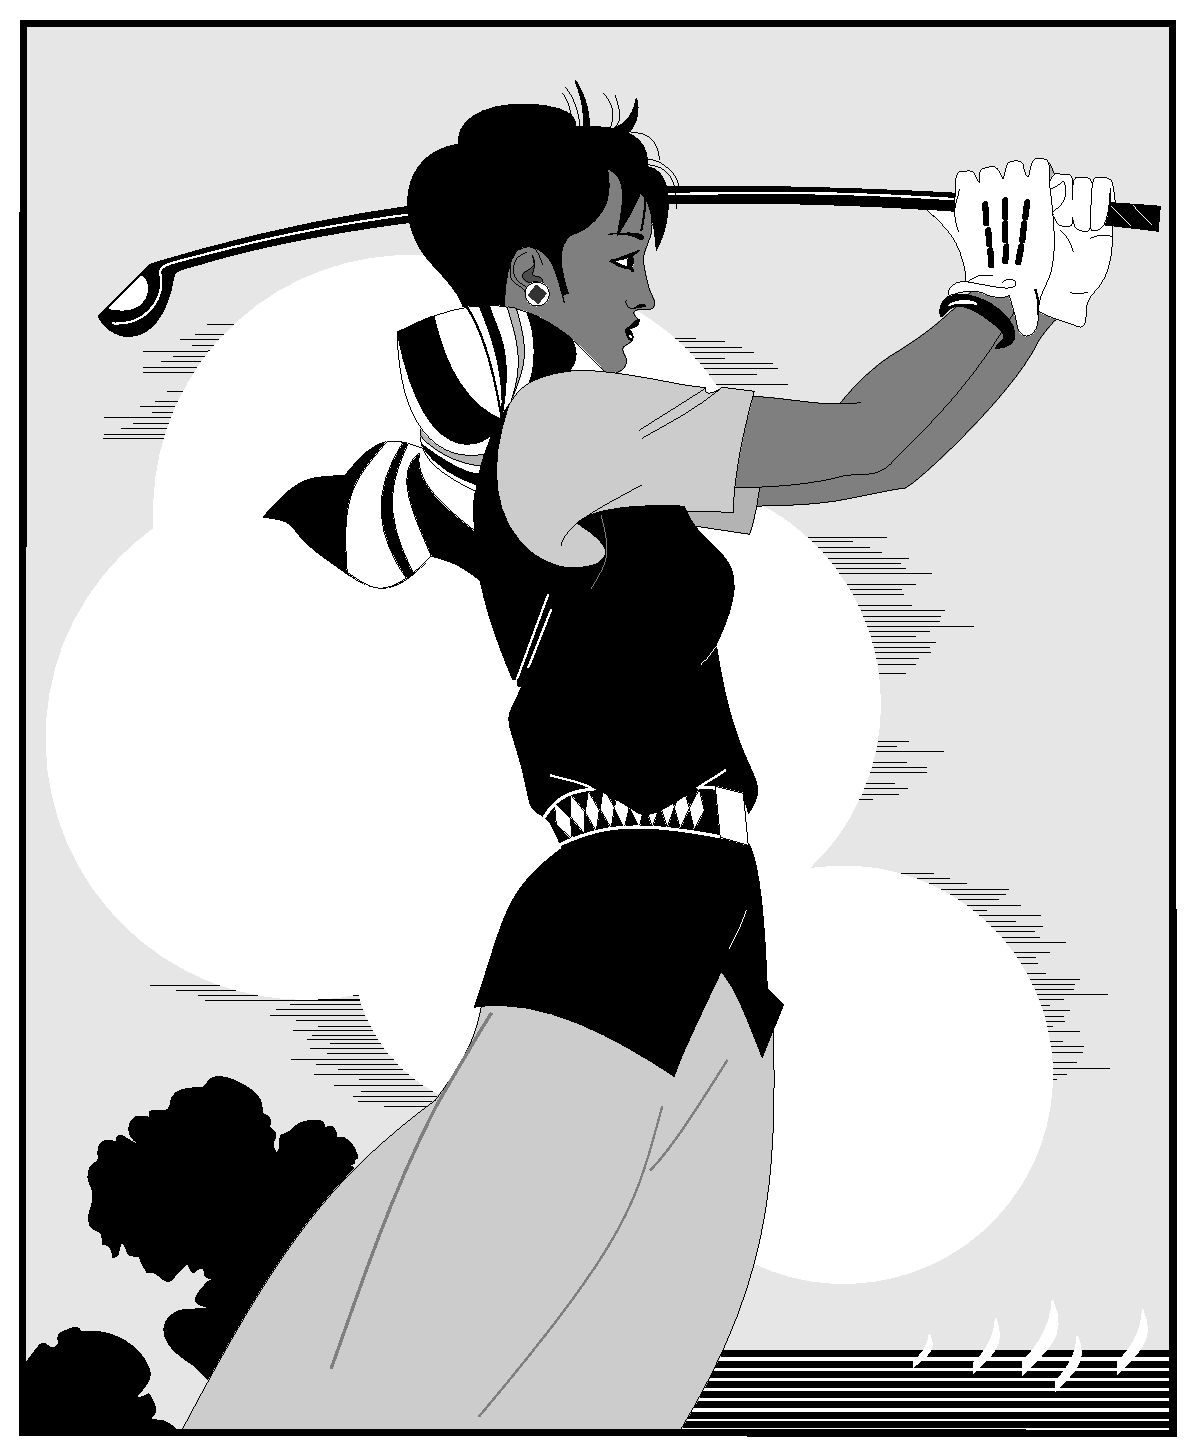
\includegraphics[width = 0.4\textwidth]{golfer}
%\bicaption[golfer5]{}{\xiaosi[0]打高尔夫球的人}{Fig.$\!$}{The person playing golf}\vspace{-1em}
\caption{\xiaosi[0]打高尔夫球的人}
\end{figure}

附录中公式的示例:
\begin{align}
a & = b \times c \\
E & = m c^2
\label{eq}
\end{align}

\chapter{这个星球上最好的免费Linux软件列表}[List of the Best Linux Software in our Planet]
\section{系统}

\href{http://fvwm.org/}{FVWM自从上世纪诞生以来,此星球最强大的窗口管理器。}
推荐基于FVWM的桌面设计hifvwm:\href{https://github.com/dustincys/hifvwm}{https://github.com/dustincys/hifvwm}。

\subsection{hifvwm的优点}

\begin{enumerate}
	\item 即使打开上百个窗口也不会“蒙圈”,对比win或mac都无法做到。计算机性能越来越强大,窗口任务的管理必须要升级到打怪兽级别。
	\item 二维可视化任务栏。
	\item 自动同步Bing搜索主页的壁纸。每次电脑开机,午夜零点自动更新,用户
		也可以手动更新,从此审美再也不疲劳。
	\item 切换窗口自动聚焦到最上面的窗口。使用键盘快捷键切换窗口时候,减少
		操作过程,自动聚焦到目标窗口。这一特性是虚拟窗口必须的人性化设
		计。
	\item 类似window右下角的功能的最小化窗口来显示桌面的功能此处类似
		win7/win10,实现在一个桌面之内操作多个任务。
	\item 任务栏结合标题栏。采用任务栏和标题栏结合,节省空间。
	\item 同类窗口切换。可以在同类窗口之内类似alt-tab的方式切换。
	\item ……
\end{enumerate}

\section{其他}

\href{https://github.com/goldendict/goldendict}{goldendict 星球最强大的桌面字典。}

\href{https://github.com/yarrick/iodine}{iodine,“HIT-WLAN + 锐捷”时代的福音。}

\href{http://www.aircrack-ng.org/}{aircrack,Wifi“安全性评估”工具,自由上网,
  就是隔壁寝室网络会变慢一点。}

\href{https://www.ledger-cli.org/}{ledger,前“金融区块链”时代最好的复式记账系统。}

\href{https://orgmode.org/}{orgmode,最强大的笔记系统,从来没有之一。}

\href{https://www.jianguoyun.com/}{坚果云,国内一款支持WebDav的云盘系统,国内真正的云盘没有之一。}

\href{https://notmuchmail.org/}{notmuch, 目前最好的邮件管理工具,还在为每天几百
  个email苦恼?几百个这些都不算多,notmuch。}

\section{vim}
实现中英文每一句一行,以及实现每一句折叠断行的简单正则式,tex源码更加乖乖。
\begin{lstlisting}
vnoremap <leader>fae J:s/[.!?]\zs\s\+/\="\r".matchstr(getline('.'), '^\s*')/g<CR>
vnoremap <leader>fac J:s/[。!?]/\=submatch(0)."\n".matchstr(getline('.'), '^\s*')/g<CR>
vnoremap <leader>fle :!fmt -80 -s<CR>
\end{lstlisting}

% \end{appendix}
% % !Mode:: "TeX:UTF-8" 
\begin{publication}
\noindent\textbf{发表的相关论文}
\begin{publist}
\item	XXX,XXX. Static Oxidation Model of Al-Mg/C Dissipation Thermal Protection Materials[J]. Rare Metal Materials and Engineering, 2010, 39(Suppl. 1): 520-524.(SCI~收录,IDS号为~669JS,IF=0.16)
\item XXX,XXX. 精密超声振动切削单晶铜的计算机仿真研究[J]. 系统仿真学报,2007,19(4):738-741,753.(EI~收录号:20071310514841)
\item XXX,XXX. 局部多孔质气体静压轴向轴承静态特性的数值求解[J]. 摩擦学学报,2007(1):68-72.(EI~收录号:20071510544816)
\item XXX,XXX. 硬脆光学晶体材料超精密切削理论研究综述[J]. 机械工程学报,2003,39(8):15-22.(EI~收录号:2004088028875)
\item XXX,XXX. 基于遗传算法的超精密切削加工表面粗糙度预测模型的参数辨识以及切削参数优化[J]. 机械工程学报,2005,41(11):158-162.(EI~收录号:2006039650087)
\item XXX,XXX. Discrete Sliding Mode Cintrok with Fuzzy Adaptive Reaching Law on 6-PEES Parallel Robot[C]. Intelligent System Design and Applications, Jinan, 2006: 649-652.(EI~收录号:20073210746529)
\end{publist}

\noindent\textbf{(二)申请及已获得的专利(无专利时此项不必列出)}
\begin{publist}
\item XXX,XXX. 一种温热外敷药制备方案:中国,88105607.3[P]. 1989-07-26.
\end{publist}

\noindent\textbf{(三)参与的科研项目及获奖情况}
\begin{publist}
\item	XXX,XXX. XX~气体静压轴承技术研究, XX~省自然科学基金项目.课题编号:XXXX.
\item XXX,XXX. XX~静载下预应力混凝土房屋结构设计统一理论. 黑江省科学技术二等奖, 2007.
\end{publist}
%\vfill
%\hangafter=1\hangindent=2em\noindent
%\setlength{\parindent}{2em}
\end{publication}
    % 所发文章
% \begin{ceindex}
  %如果想要手动加索引,注释掉以下这一样,用wordlist环境
\printsubindex*
\end{ceindex}
    % 索引, 根据自己的情况添加或者不添加,选择自动添加或者手工添加。
% \authorization %授权
% %\authorization[scan.pdf] %添加扫描页的命令,与上互斥
% % !TEX root = ../main.tex

% 致谢
\begin{acknowledgements}
衷心感谢导师~XXX~教授对本人的精心指导。他的言传身教将使我终生受益。

……

感谢哈深\LaTeX{}论文模板\hitszthesis\ !

\end{acknowledgements}
 %致谢
% % !TEX root = ../main.tex

% 个人简历
\begin{resume}

  XXXX~年~XX~月~XX~日出生于~XXXX。

  XXXX~年~XX~月考入~XX~大学~XX~院(系)XX~专业,XXXX~年~XX~月本科毕业并获得~XX~学学士学位。

  XXXX~年~XX~月------XXXX~年~XX~月在~XX~大学~XX~院(系)XX~学科学习并获得~XX~学硕士学位。

  XXXX~年~XX~月------XXXX~年~XX~月在~XX~大学~XX~院(系)XX~学科学习并获得~XX~学博士学位。

  获奖情况:如获三好学生、优秀团干部、X~奖学金等(不含科研学术获奖)。

  工作经历:

  \songti\textbf{(除全日制硕士生以外,其余学生均应增列此项。个人简历一般应包含教育经历和工作经历。)}

\end{resume}
          % 博士学位论文有个人简介
%%%%%%%%%%%%%%%%%%%%%%%%%%%%%%%%%%%%%%%%%%%%%%%%%%%%%%%%%%%%%%%%%%%%%%%%%%%%%%%%
% 博后书序
%%%%%%%%%%%%%%%%%%%%%%%%%%%%%%%%%%%%%%%%%%%%%%%%%%%%%%%%%%%%%%%%%%%%%%%%%%%%%%%%
% \bibliography{reference} % 参考文献
% % !TEX root = ../main.tex

% 致谢
\begin{acknowledgements}
衷心感谢导师~XXX~教授对本人的精心指导。他的言传身教将使我终生受益。

……

感谢哈深\LaTeX{}论文模板\hitszthesis\ !

\end{acknowledgements}
 %致谢
% % !Mode:: "TeX:UTF-8" 

\begin{doctorpublication}
\noindent\textbf{(一)发表的学术论文}
\begin{publist}
\item	XXX,XXX. Static Oxidation Model of Al-Mg/C Dissipation Thermal Protection Materials[J]. Rare Metal Materials and Engineering, 2010, 39(Suppl. 1): 520-524.(SCI~收录,IDS号为~669JS,IF=0.16)
\item XXX,XXX. 精密超声振动切削单晶铜的计算机仿真研究[J]. 系统仿真学报,2007,19(4):738-741,753.(EI~收录号:20071310514841)
\item XXX,XXX. 局部多孔质气体静压轴向轴承静态特性的数值求解[J]. 摩擦学学报,2007(1):68-72.(EI~收录号:20071510544816)
\item XXX,XXX. 硬脆光学晶体材料超精密切削理论研究综述[J]. 机械工程学报,2003,39(8):15-22.(EI~收录号:2004088028875)
\item XXX,XXX. 基于遗传算法的超精密切削加工表面粗糙度预测模型的参数辨识以及切削参数优化[J]. 机械工程学报,2005,41(11):158-162.(EI~收录号:2006039650087)
\item XXX,XXX. Discrete Sliding Mode Cintrok with Fuzzy Adaptive Reaching Law on 6-PEES Parallel Robot[C]. Intelligent System Design and Applications, Jinan, 2006: 649-652.(EI~收录号:20073210746529)
\end{publist}

\noindent\textbf{(二)申请及已获得的专利(无专利时此项不必列出)}
\begin{publist}
\item XXX,XXX. 一种温热外敷药制备方案:中国,88105607.3[P]. 1989-07-26.
\end{publist}

\noindent\textbf{(三)参与的科研项目及获奖情况}
\begin{publist}
\item	XXX,XXX. XX~气体静压轴承技术研究, XX~省自然科学基金项目.课题编号:XXXX.
\item XXX,XXX. XX~静载下预应力混凝土房屋结构设计统一理论. 黑江省科学技术二等奖, 2007.
\end{publist}
%\vfill
%\hangafter=1\hangindent=2em\noindent
%\setlength{\parindent}{2em}
\end{doctorpublication}
    % 所发文章
% % !Mode:: "TeX:UTF-8" 
\begin{publication}
\noindent\textbf{发表的相关论文}
\begin{publist}
\item	XXX,XXX. Static Oxidation Model of Al-Mg/C Dissipation Thermal Protection Materials[J]. Rare Metal Materials and Engineering, 2010, 39(Suppl. 1): 520-524.(SCI~收录,IDS号为~669JS,IF=0.16)
\item XXX,XXX. 精密超声振动切削单晶铜的计算机仿真研究[J]. 系统仿真学报,2007,19(4):738-741,753.(EI~收录号:20071310514841)
\item XXX,XXX. 局部多孔质气体静压轴向轴承静态特性的数值求解[J]. 摩擦学学报,2007(1):68-72.(EI~收录号:20071510544816)
\item XXX,XXX. 硬脆光学晶体材料超精密切削理论研究综述[J]. 机械工程学报,2003,39(8):15-22.(EI~收录号:2004088028875)
\item XXX,XXX. 基于遗传算法的超精密切削加工表面粗糙度预测模型的参数辨识以及切削参数优化[J]. 机械工程学报,2005,41(11):158-162.(EI~收录号:2006039650087)
\item XXX,XXX. Discrete Sliding Mode Cintrok with Fuzzy Adaptive Reaching Law on 6-PEES Parallel Robot[C]. Intelligent System Design and Applications, Jinan, 2006: 649-652.(EI~收录号:20073210746529)
\end{publist}

\noindent\textbf{(二)申请及已获得的专利(无专利时此项不必列出)}
\begin{publist}
\item XXX,XXX. 一种温热外敷药制备方案:中国,88105607.3[P]. 1989-07-26.
\end{publist}

\noindent\textbf{(三)参与的科研项目及获奖情况}
\begin{publist}
\item	XXX,XXX. XX~气体静压轴承技术研究, XX~省自然科学基金项目.课题编号:XXXX.
\item XXX,XXX. XX~静载下预应力混凝土房屋结构设计统一理论. 黑江省科学技术二等奖, 2007.
\end{publist}
%\vfill
%\hangafter=1\hangindent=2em\noindent
%\setlength{\parindent}{2em}
\end{publication}
    % 所发文章
% % !TEX root = ../main.tex

% 个人简历
\begin{resume}

  XXXX~年~XX~月~XX~日出生于~XXXX。

  XXXX~年~XX~月考入~XX~大学~XX~院(系)XX~专业,XXXX~年~XX~月本科毕业并获得~XX~学学士学位。

  XXXX~年~XX~月------XXXX~年~XX~月在~XX~大学~XX~院(系)XX~学科学习并获得~XX~学硕士学位。

  XXXX~年~XX~月------XXXX~年~XX~月在~XX~大学~XX~院(系)XX~学科学习并获得~XX~学博士学位。

  获奖情况:如获三好学生、优秀团干部、X~奖学金等(不含科研学术获奖)。

  工作经历:

  \songti\textbf{(除全日制硕士生以外,其余学生均应增列此项。个人简历一般应包含教育经历和工作经历。)}

\end{resume}
          % 博士学位论文有个人简介
% % !Mode:: "TeX:UTF-8"
\begin{correspondingaddr}
  \heiti\xiaosi
  \noindent 永久通讯地址: \par
  \noindent email: \par
  \noindent 电话: \par
\end{correspondingaddr}
 %通信地址
%%%%%%%%%%%%%%%%%%%%%%%%%%%%%%%%%%%%%%%%%%%%%%%%%%%%%%%%%%%%%%%%%%%%%%%%%%%%%%%%
\end{document}
% Local Variables:
% TeX-engine: xetex
% End:
